%%
%% This is file `team-eagle-lazer-fang.tex',
%%
%% A modified copy of:
%%
%% sample-authordraft.text
%% 
%% IMPORTANT NOTICE:
%% 
%% For the copyright see the source file.
%% 
%% Any modified versions of this file must be renamed
%% with new filenames distinct from sample-manuscript.tex.
%% 
%% For distribution of the original source see the terms
%% for copying and modification in the file samples.dtx.
%% 
%% This generated file may be distributed as long as the
%% original source files, as listed above, are part of the
%% same distribution. (The sources need not necessarily be
%% in the same archive or directory.)
%%
%% The first command in your LaTeX source must be the \documentclass command.
%%%% Small single column format, used for CIE, CSUR, DTRAP, JACM, JDIQ, JEA, JERIC, JETC, PACMCGIT, TAAS, TACCESS, TACO, TALG, TALLIP (formerly TALIP), TCPS, TDSCI, TEAC, TECS, TELO, THRI, TIIS, TIOT, TISSEC, TIST, TKDD, TMIS, TOCE, TOCHI, TOCL, TOCS, TOCT, TODAES, TODS, TOIS, TOIT, TOMACS, TOMM (formerly TOMCCAP), TOMPECS, TOMS, TOPC, TOPLAS, TOPS, TOS, TOSEM, TOSN, TQC, TRETS, TSAS, TSC, TSLP, TWEB.
% \documentclass[acmsmall]{acmart}

%%%% Large single column format, used for IMWUT, JOCCH, PACMPL, POMACS, TAP, PACMHCI
% \documentclass[acmlarge,screen]{acmart}

%%%% Large double column format, used for TOG
% \documentclass[acmtog, authorversion]{acmart}

%%%% Generic manuscript mode, required for submission
%%%% and peer review
\documentclass[manuscript,screen,review]{acmart}

\usepackage{tikz}
\usetikzlibrary{shapes.geometric, arrows, patterns}
\usepackage{graphicx}
\usepackage{subcaption}
% \usepackage{draftwatermark}
% \SetWatermarkText{\includegraphics[width = 0.25\textwidth, opacity = 0.1]{graphics/Untitled-1.png}}
%% Fonts used in the template cannot be substituted; margin 
%% adjustments are not allowed.
%%
%% \BibTeX command to typeset BibTeX logo in the docs
\AtBeginDocument{%
  \providecommand\BibTeX{{%
    \normalfont B\kern-0.5em{\scshape i\kern-0.25em b}\kern-0.8em\TeX}}}

%% Rights management information.  This information is sent to you
%% when you complete the rights form.  These commands have SAMPLE
%% values in them; it is your responsibility as an author to replace
%% the commands and values with those provided to you when you
%% complete the rights form.
% \setcopyright{acmcopyright}
% \copyrightyear{2018}
% \acmYear{2018}
% \acmDOI{XXXXXXX.XXXXXXX}

% %% These commands are for a PROCEEDINGS abstract or paper.
% \acmConference[Conference acronym 'XX]{Make sure to enter the correct
%   conference title from your rights confirmation emai}{June 03--05,
%   2018}{Woodstock, NY}
% %
% %  Uncomment \acmBooktitle if th title of the proceedings is different
% %  from ``Proceedings of ...''!
% %
% \acmBooktitle{Woodstock '18: ACM Symposium on Neural Gaze Detection,
%  June 03--05, 2018, Woodstock, NY} 
% \acmPrice{15.00}
% \acmISBN{978-1-4503-XXXX-X/18/06}


%%
%% Submission ID.
%% Use this when submitting an article to a sponsored event. You'll
%% receive a unique submission ID from the organizers
%% of the event, and this ID should be used as the parameter to this command.
%%\acmSubmissionID{123-A56-BU3}

%%
%% The majority of ACM publications use numbered citations and
%% references.  The command \citestyle{authoryear} switches to the
%% "author year" style.
%%
%% If you are preparing content for an event
%% sponsored by ACM SIGGRAPH, you must use the "author year" style of
%% citations and references.
%% Uncommenting
%% the next command will enable that style.
\citestyle{acmauthoryear}

%%
%% end of the preamble, start of the body of the document source.
\begin{document}

%%
%% The "title" command has an optional parameter,
%% allowing the author to define a "short title" to be used in page headers.
\title{Trustworthiness of AI decision making tools in high-risk applications.} % Impact of model transparency on stakeholder trust in high-stakes scenarios

%%
%% The "author" command and its associated commands are used to define
%% the authors and their affiliations.
%% Of note is the shared affiliation of the first two authors, and the
%% "authornote" and "authornotemark" commands
%% used to denote shared contribution to the research.
\author{Alex Davies}
\affiliation{%
  \institution{Interactive AI CDT, University of Bristol}
  \country{UK}
}
\author{Daniel Collins}
\affiliation{%
  \institution{Interactive AI CDT, University of Bristol}
  \country{UK}
}
\author{Isabella Degen}
\affiliation{%
  \institution{Interactive AI CDT, University of Bristol}
  \country{UK}
}
\author{Jonathan Erskine}
\affiliation{%
  \institution{Interactive AI CDT, University of Bristol}
  \country{UK}
}
\author{Matt Clifford}
\affiliation{%
  \institution{Interactive AI CDT, University of Bristol}
  \country{UK}
}
\author{Ronja Spaniel}
\affiliation{%
  \institution{Interactive AI CDT, University of Bristol}
  \country{UK}
}

%%
%% By default, the full list of authors will be used in the page
%% headers. Often, this list is too long, and will overlap
%% other information printed in the page headers. This command allows
%% the author to define a more concise list
%% of authors' names for this purpose.
\renewcommand{\shortauthors}{Team Eagle Lazer Fang, et al.}

%%
%% The abstract is a short summary of the work to be presented in the
%% article.
\begin{abstract}
%Include motivation and Contribution
%what's our contribution - first sentence
%why are we doing this research -> one sentence
%mention survey of x people and focus group -> one sentence on what we did
%what have we done - why is it new - how have we done it - what are our findings (short)
 
An abundance of new methods explaining how Artificial Intelligence has made a decision have been created in the last few years. These explanations endeavour to make AI decision making more transparent and increase the trust humans place into AI decision making. There's a lack of research into how well explainable AI serves the needs of people who are affected by the decisions of an AI system and if it indeed increases their trust. In this study we asked $n=278$ people in an online survey how much they would trust a diagnosis of having COVID or not made in four different scenarios: (1) a doctor on their own, (2) a interpretable AI system (Glass box) with the Dr, (3) an AI system that's not interpretable (Black Box) with the Dr and (4) a Black Box AI system on its own. The survey participants also specified their expertise in AI, if their working in health care or not as well as how frequent they are making high-stakes decisions (decisions that could impact the lives of others). We followed the survey up with a focus group of 6 participants to discuss the topic further. We found that people impacted by an AI system making a medical diagnosis trust a glass box AI system working with a doctor the most and a black box AI system working by itself the least. People who make frequent high-stakes decisions trust a doctor on their own the least. People who report having medium or high AI experience trust the black box working with the Dr more and people who don't work in healthcare trust the black box less than other demographics. Surprisingly when ranked the Dr working on their own was across the demographics second most frequently ranked the lowest while at the same time being second most frequently ranked the highest in trust. Finally we found that the dislike of the black box has less to do with the lack of interpretablity and more to do with the lack of empathy when a machine diagnoses someone with a potential severe illness.
\end{abstract}

%%
%% The code below is generated by the tool at http://dl.acm.org/ccs.cfm.
%% Please copy and paste the code instead of the example below.
%%
% \begin{CCSXML}
% <ccs2012>
%  <concept>
%   <concept_id>10010520.10010553.10010562</concept_id>
%   <concept_desc>Computer systems organization~Embedded systems</concept_desc>
%   <concept_significance>500</concept_significance>
%  </concept>
%  <concept>
%   <concept_id>10010520.10010575.10010755</concept_id>
%   <concept_desc>Computer systems organization~Redundancy</concept_desc>
%   <concept_significance>300</concept_significance>
%  </concept>
%  <concept>
%   <concept_id>10010520.10010553.10010554</concept_id>
%   <concept_desc>Computer systems organization~Robotics</concept_desc>
%   <concept_significance>100</concept_significance>
%  </concept>
%  <concept>
%   <concept_id>10003033.10003083.10003095</concept_id>
%   <concept_desc>Networks~Network reliability</concept_desc>
%   <concept_significance>100</concept_significance>
%  </concept>
% </ccs2012>
% \end{CCSXML}

% \ccsdesc[500]{Computer systems organization~Embedded systems}
% \ccsdesc[300]{Computer systems organization~Redundancy}
% \ccsdesc{Computer systems organization~Robotics}
% \ccsdesc[100]{Networks~Network reliability}

%%
%% Keywords. The author(s) should pick words that accurately describe
%% the work being presented. Separate the keywords with commas.
\keywords{XAI, Explainable AI, Trustworthy AI, Interpretable AI, attitudes towards AI, automated decision making, AI in healthcare}

%%
%% This command processes the author and affiliation and title
%% information and builds the first part of the formatted document.
\maketitle

\newpage
\section{Introduction}\label{sec:introduction}
%%%%%%%%%%%
% Keeping notes from previous list making
%%%%%%%%%%%
%Motivate the research
%give an overview of relevant background literature
%describe the research question.
%Possibly signpost the findings
% notes on how to writing
% go straight to the point
% don't make it so general that it could be used for an other paper
% don't slash others works
% include problem / solution

%Initial structure:
%\begin{itemize}
%    \item AI used in many use applications (give examples of high risk etc) - we focused on healthcare
%    \item For successful integration of AI, users and public need to trust it. 
%    \item Law came into that decisions for banks etc needed to be explained to the user, the right to explanation, e.g GDPR %https://www.turing.ac.uk/research/impact-stories/a-right-to-explanation
%    \item this brought about interest in XAI (Why XAI has been seen as important (Issues with this - black box models, not always human able to intervene/oversee))
%    \item Lots of work has been done into XAI techniques to give `trust' in AI.
%    \item XAI examples to show off the amount of work been done  - survey papers and specific examples? LIME? FATF?
%    \item Issues with XAI - critics (to give some doubt over XAI actually giving trust and telling us how AI works)
%    \item Is the current work in XAI just useful for machine learning practitioners? 
%    \item What is best for the users/ what do users actually want? Has the explanation law confused us of what users actually want/need?
%    \item We want to explore what trust actually is in relation to AI. Is it XAI? Is it performance? Is it counterfactual results? (are they more intuitive/what people would like to know)?
%    \item There has been the topic of trust between humans and machines before (1987 paper). Which indicates that there needs to be trust not just performance.
%    \item There is no current user study of how XAI changes trust depending on: demographic (AI expert, high stakes decision maker, general public) or the level of explainablity. 
%    % \item medical domain - paper Alex found on simple AI in a medical context out-performing doctors
%\end{itemize}
%Ann's suggestion of structure:
%\begin{itemize}
%    \item Context (how is the world now): Messy, AI and Explainable AI, 
%    \item the problem (drama): loads of research, not many survey on what's needed on trust, does transparency and explainable creates more or less trust
%    \item related work and how it doesn't cover this: GDPR has created a flood of research into Explainable AI, so it's not been questioned much on the motivations. Surveys on trust in generic AI systems. Surveys of perspectives on generic AI system for healthcare work groups.
%    \item our solution, method and results: survey and focus group to find out if trust increases with transparency and if experience with AI or high stakes decision making matters
%    \item what new worlds does our research do: design with all demographics in mind, different branches of explainability. Present information that can be used to design better AI systems for healthcare needs. Encourage more user driven explainable AI with the demographics we find
%\end{itemize}

% Isabella: I've kept the bullet points for the text below in my google doc if needed
%%%%%%%%%%%%%%%%


% Why Context - how is the world now
AI is being deployed in a variety of different domains, including high-risk application areas where algorithms are potentially making life-altering decisions; including applications in insurance, criminal justice and healthcare \cite{Bohr2020}, \cite{Chen2018}. It is widely believed that new laws like the EU General Data Protection Regulation (GDPR) mandate a ‘right to explanation’ as a mechanism to enhance the accountability and transparency of automated decision-making \cite{Wachter2017}. While that right does not explicitly exist \cite{Wachter2017}, the approval of the GDPR in 2016 created an explosion of research in Explainable AI (XAI) and closely related research areas such as: Transparent AI, Interpretable AI and Trustworthy AI. The desired outcome of these research areas is to create responsible and ethical AI systems that are fair and allow for accountability \cite{Mohseni2021}, often referred to as Responsible AI. This has led to a surge of new methods that explain the decisions of different AI algorithms, see \cite{Linardatos2021} and \cite{Guidotti2018a} for an overview. This abundance of new methods has given rise to endeavours to standardise and asses the quality of explanations see \cite{Gilpin2019}. Other works have attempted to create an unified and standardised taxonomy and definitions for explainable, transparent, interpretable and trustworthy AI \cite{Schwalbe2021} and \cite{Arrieta2020}.

%Why new - The problem (drama)
The huge increase in the popularity of explainable, interpretable and trustworthy AI has in turn given rise to debate. The motivations behind explainable AI, the quality \cite{Doshi-Velez2017} and usefulness of the explanations given \cite{Miller2019}, as well as whether explainable AI achieves its objective of higher trust in AI \cite{Lipton2018}, are ongoing areas of research. Research into explainable AI recognises that there are many different stakeholders of AI systems, including developers, end-users and lawmakers. The needs of each of these stakeholders vary greatly. 

For the developers of AI systems the explanations are useful for evaluating, testing and debugging purposes. They have a deep and technical understanding of the concepts and mathematics behind the algorithms and are therefore able to interpret mathematical explanations of those systems. These are the people who are creating new explainability methods and we refer to them as AI experts \cite{Carvalho2019}.

The end users of the AI systems are people who use these systems in their work e.g clinicians. They are domain experts in the problem that the AI system solves. These end users are interested in explanations to help them assess the model’s decision and decide on the actions to be taken. Examples of research into how well their needs are served with interpretable and explainable AI can be found in \cite{Goldstein2021}, \cite{Liao2020}, and \cite{Salimiparsa2021}.

The final stakeholders are the people who are affected by the decision of an AI system, for example for example patients that are being diagnosed by an AI system. However, there is a lack of research into how well their needs are being served by explainable AI and if they need more transparent and explainable AI systems to better trust AI.

%more related work
A study surveyed 922 women’s attitude toward AI in mammography screening. They found that they preferred a combination of radiologist and AI system \cite{Ongena2021}. Another study surveyed 216 fracture patients on their perceptions towards AI used to assist in interpretation of their radiographs and found that participant’s held the clinician’s assessment in the highest regard \cite{York2020}. A further study found that patients are apprehensive about the use of AI \cite{Richardson2021} and highlighted the need for early patient involvement in the AI systems being used in healthcare. These studies did not investigate the role that transparency and performance of the AI system played in the patients attitudes.

% more related work and how it doesn't cover this: Surveys on trust in generic AI systems. Surveys of perspectives on generic AI systems for healthcare work groups.
There is no current user study of how XAI changes trust depending on: demographic (AI expert, high stakes decision maker, general public) nor the level of explainability.  

%What & How: our solution, method and results: survey and focus group to find out if trust increases with transparency and if experience with AI or high stakes decision making matters
In this study we are focusing on the opinions of people who are affected by the decision of an AI system. We created a survey of $n=278$ people who were asked to imagine being diagnosed in a hospital whether they have COVID or not in four different scenarios:

\begin{enumerate}
    \item A doctor makes the diagnosis.
    \item A doctor makes the diagnosis together with an interpretable AI system (a so called glass box system).
    \item A doctor makes the diagnosis together with an AI system that’s not interpretable (a so called black box system).
    \item A black box system makes the diagnosis by itself.
\end{enumerate}

For each of these scenarios the participants were told how often the doctor and AI system make the correct diagnosis (the performance) and how much the doctor knew about why the AI system made its decision (the interpretability of the system). The participants were asked to express how much they would trust to be diagnosed by that setup by selecting a number from 1-10. We furthermore collected demographic information about the participants, namely if they are working in healthcare or not, how much experience and knowledge they have about AI as well as how frequently they are making high-stakes decisions (life-altering decisions). The scenarios were designed in such a way that of the patients who have Covid the doctor and glass box both correctly diagnose 85 out of 100 while the black box had a significantly better performance of 95 correct diagnoses out of 100. This is an equivalent to a "true positive rate" in information science, or "sensitivity" in medicine, which are accepted measures of performance in both fields.

We analysed the responses with regards to which scenario was trusted the most respectively least and how this changed depending on the participants demographic. We found that the black box on its own was the least trusted scenario and the doctor working together with the glass box was the most trusted scenario. Surprisingly and contradictory to what other research has found when ranking the four different scenarios, the Dr on their own was the second most frequent lowest ranked scenario, and also the second most frequent highest ranked scenario. The doctor working with the black box gained  more trust than the black box on its own. The demographic of the participants did not change this ranking with the exceptions of participants that reported making frequent high stakes decisions, they ranked the doctor by themselves the lowest. Furthermore, participants with medium and high AI expertise trust the doctor with the black box more than participants with low AI expertise. Finally, participants who work in healthcare either trust the doctor by itself a lot or not at all, while participants who don’t work in healthcare trust the black box by itself less.

We followed the survey up with a focus group of 6 people to discuss and reflect further on their thoughts about AI and the need for interpretability and explanations as well as exploring if black box models will ever be accepted. We found that the dislike of the black box has less to do with the lack of interpretablity, but more to do with the lack of empathy that a machine can give compared to a human when diagnosing someone with a potential critical illness. However, the focus group rated the black box higher than the survey participant did under the conditions that it had high performance and that the patient had full disclosure of a black box being used or that it was used in a low-stakes application area.


%Why relevant: what new worlds does our research do: design with all demographics in mind, different branches of explainability. Present information that can be used to design better AI systems for healthcare needs. Encourage more user driven explainable AI with the demographics we find
<todo> We believe that for an AI system to be adapted in a critical decision scenario, such as diagnosis in health care, it is not sufficient to just make the system transparent and explainable. It is far more important to complete the user experience and give an understanding that the AI system is only a part of that experience. We believe that more research is needed to understand this area fully.\\

The current techniques are useful for the operators of the systems, however, the law is to protect the end user that is affected by an AI having been used. It is clear that the needs for these groups are different and more research needs to be done to consider the end users of those systems and what their needs are and how they differ from the operators.\\

\newpage
\section{Related Work}\label{sec:related-work}
%Outline:
%
% What is Explainable AI
% What is interpretable AI
% What is transparency AI
% What is trustwortiness in AI
% Why is Explainable AI needed
% How is XAI different in Healtcare
% Shortfalls and critique of XAI, how XAI is not needed, include critics of HCI, difficulties of too many stakehoders
%
% Where do the methods go? Do they fit here

\subsection{An overview of transparent, interpretable and explainable AI}\label{subsec:an-overview-of-transparent-interpretable-and-explainable-ai}
The field of explainable AI (XAI) experienced a huge surge since 2016 an there is no shortage of surveys of the research.

The literature speaks of black and glass box (also called white box) systems.
Black box models are complex systems that are not transparent.
It is not clear to a human how and why the system makes a decision.
On the other hand glass boxes models are systems that are interpretable and transparent by default.
Explanations can be seen as adding a form of post-hoc interpretability to an AI system and with that make AI models more transparent with regards to how they make decisions.
There's a wide variety of terminologies, motivations, approaches and evaluation criteria for XAI methods.
Many researchers have created surveys of these methods and attempted to create a unified taxonomies \cite{Linardatos2021} and\cite{Schwalbe2021}.
However, despite the vast body of knowledge developed around the concept of explainability, there is not a general consensus among scholars on how an explanation should be defined, or how its validity and reliability should be assessed\cite{Vilone2021}.

There are also many surveys that focus on summarizing the available explanation methods such as\cite{Vilone2020},
a field guide of explainable AI for Deep Learning\cite{Ras2020}, a survey of methods for explaining black box models\cite{Guidotti2018a} \&\cite{Adadi2018},
a survey of post-hoc explanation by example methods\cite{Keane2019}, contrastive explanations\cite{Miller2021},
explanations using counterfactuals\cite{Verma2020} \&\cite{Keane2020}, rule based explanations\cite{Guidotti2018} as well
as conversational explanations\cite{Sokol2018}.

Note that this recent wave of explanations of automated decision making is not the first wave.
An earlier wave happened around automated decision making in control systems as well as AI in the late 1980s see\cite{Chandrasekaran1989}.

\subsection{Why Explainable AI is needed}\label{subsec:why-explainable-ai-is-needed}

Gunning 2018 states:
\begin{quote}
    \textit{"Explainability is essential for users to effectively understand, trust, and manage powerful artificial intelligence applications."}  \cite{Gunning2019}
\end{quote}

Bansal and co studied if explanations increase the performance of the human-AI team and found that this was not the case.
Instead they found that the explanations increased the chance that the human will accept the AI's recommendation regardless of the correctness thereof.
Their findings suggest that explanations increase trust in AI\cite{Bansal2020}.

Weld and co found that to trust an AI system's behavior, it must be intelligible, either by using inherently interpretable models or by developing new methods for explaining and controlling otherwise overwhelmingly complex decisions using local approximation, vocabulary alignment, and interactive explanation \cite{Weld2019}.


\subsection{Shortfalls and Critics of current XAI}\label{subsec:shortfalls-and-critics-of-current-xai}

XAI has also received a fair amount of critique.
From questioning if explainability and interpretability can be achieved to the vague definitions of the terms used \cite{Lipton2018}.

Researchers have also been starting to investigate if supposedly interpretable models achieve their intended effects, such as making people more closely follow a model's predictions when it is beneficial for them to do so or enabling them to detect when a model has made a mistake.
They however did not find that participants more closely followed its predictions\cite{Goldstein2021}.

Ehsan and co argue that explanations need to be more human centered.
Building on their case study they stress that more focus on the human is needed and that technical advancements and the understanding of human factors co-evolve together.\cite{Ehsan2020}

However, exactly what kinds of explanation are truly human-interpretable remains poorly understood.
This work advances our understanding of what makes explanations interpretable in the specific context of verification.
In general, greater complexity results in higher response times and lower satisfaction \cite{Narayanan2018}.

Felzmann and co explore what the requirement of transparency in the GDPR entails for AI and automated decision-making systems integrating integrating legal, social, and ethical aspects.
They highlight how human–computer interaction and human-robot interaction literature do not provide clear results with respect to the benefits of transparency for users of artificial intelligence technologies
and propose a relational concept of transparency. 
They suggest attention needs to be paid to factors that make transparency meaningful and trustworthy in the users’ eyes \cite{Felzmann2019}.

Markus et. al. 2021 find that evidence of the usefulness of explainability is still lacking in practice and recognize that complementary measures might be needed to create trustworthy AI \cite{Markus2021}.


\subsection{Connecting Human Computer Interaction and XAI}\label{subsec:human-computer-interaction-focused-xai}

Mohsensi and co's research created a framework to support diverse design goals and evaluation methods in XAI research \cite{Mohseni2021}.

Wang and co created a framework based on decision making and reasoning theory for AI explanation techniques.
They aim to help developers build human-centric explainable AI-based systems with targeted XAI features \cite{Wang2019}.

Amershi and co proposed and evaluated 18 generally applicable design guidelines for human-AI interaction that they hope will result in better, more human-centric AI-infused systems. 
These guidelines include principles relevant to our study such as "Make clear why the system did what it did" as well as "Make clear how well the system can do what it can
do" \cite{Amershi2019}.

Researchers from the HCI communities are interested in how to empower people and ensure that new and powerful AI technologies are designed with intelligibility from the ground up.
They highlight that while researchers in the ML and AI communities are working on making their algorithms explainable, their focus is not on usable, practical and effective transparency that works for and benefits people.
And stress that explainable systems can only be created through interdisciplinary collaborations, where expertise from different fields (e.g., machine learning, cognitive psychology, human computer interaction) is combined and concepts and techniques are further developed from multiple perspectives to move research forward.\cite{Abdul2018}

\subsection{Trust in automated decision making}\label{subsec:trust}

Trust has long been recognised as an important factor in facilitating Human Computer Interaction\cite{Lee2008}.
In the social sciences trust is studied between humans.
It's that body of work that the study of trust of humans in machines relies on.
Long before the recent AI summer, research has been done into understanding the nature of trust between humans and machines and how its important to consider what grows and diminishes trust when designing decision aids to avoid the machine's decision being rejected regardless from how sophisticated or "intelligent" it is \cite{Muir1987}.
In her research Muir also discusses that a machine needs to be designed in such a way that the user can perceive it's trustworthiness\cite{Muir1987}.
Building AI systems that are interpretable and or can explain their decision is perhaps away for a user to be able to perceive the algorithms' trustworthiness.
Despite extensive research, trust remains hard to define and there are contradicting findings and suggestions.

Many researchers agree that the performance of the decision making machine alone is not sufficient to build trust.
Muir suggests that while the machine needs to be designed well the human using it might need to recalibrate their trust in the machine's decision too \cite{Muir1987}.
Hoff and co identify three layers of variability in human–automation trust: dispositional trust, situational trust, and learned trust.
Additionally they identify also environmental conditions that can affect the strength of the relationship between trust and reliance\cite{Hoff2015}.
On the other hand Hancock and co found that a robot's performance and attributes were the largest contributors to the development of trust in human robot interaction and that environmental factors played only a moderate role.
They also state that there is little evidence for effects of human-related factors\cite{Hancock2011}.

More recently researcher have specifically looked at trust and AI.
Toreini and co and they to rely on trust as a notion within the social sciences. They show that Fair, Explainable, Auditable and Safe technologies need to be considered in the various stages of an AI system's life cycle and with that form a Chain of Trust required for trustworthy machine-learning \cite{Toreini2020}.

Chen argues that for trust to exist a set of conditions need to be satisfied.
He suggests that trust needs to be engineered either through involving a certain reliance on a set of physiognomic biases or by relying on a set of esteem-seeking psychological mechanisms. While this "Trust-Engineering" will not fully achieve trustworthy AI he argues it will ensure that reliance-without-trust can be avoided\cite{Chen2021}.
Finally Ferrario and co developed a multi-layer model of trust for human AI interaction\cite{Ferrario2020}.

\subsection{AI and XAI in healthcare}\label{subsec:ai-in-healthcare}

For this study we focus on diagnostic decisions in healthcare settings. There's evidence that public disagreement/agreement with using AI varied depending on the application area\cite{Ikkatai2022}.
Holzinger and co argue that research in explainable-AI helps to facilitate the implementation of AI/ML in the medical domain, and specifically helps to facilitate transparency and trust\cite{Holzinger2017}.
As we've mentioned earlier explanation are useful to find out if the system has learned something about medical pathology or not.
This has been demonstrated by DeGrave, they found a deep learning system used to detect COVID-19 from chest radiographs relied on confounding factors rather than medical pathology, creating an alarming situation in which the system appear accurate despite not having learned anything about medical pathology.
They conclude that their findings demonstrate that explainable AI should be seen as a prerequisite to clinical deployment of machine-learning healthcare models \cite{DeGrave2021}.

In their literature survey Nazar and co make the point of how explainable AI connects AI with Human Computer Interaction (HCI).
They also stress that more research is needed into AI and XAI in healthcare.
The hope is that explanations can be compared and validated with clinical knowledge and through that new clinical knowledge can be created or AI decisions corrected \cite{Nazar2021}.

There is also research showing that AI can be used for diagnosing Covid.
Guefrechi and co show transfer learning proves to be effective, showing strong performance and easy-to-deploy COVID-19 detection methods.
This enables automatizing the process of analyzing X-ray images with high accuracy and it can also be used in cases where the materials and RT-PCR tests are limited\cite{Guefrechi2021}.

The needs depending on the stakeholders in healthcare also change.
Medical physicist are the end-users.
Diaz and co investigated their current perceptions, practices and education needs and found that while the value of AI is recognised by medical physicists, more training of the operators of the system is needed.
They also conclude that medical physicists should be more included in AI projects\cite{Diaz2021}.

%we could move these papers to the discussion:
The patients' view on the implementation of artificial intelligence in radiology is still mainly unexplored territory.
Ongena and co found the following 5 factors mattered the most: (1) distrust and accountability (overall, patients were moderately negative on this subject), (2) procedural knowledge (patients generally indicated the need for their active engagement), (3) personal interaction (overall, patients preferred personal interaction), (4) efficiency (overall, patients were ambiguous on this subject), and (5) being informed (overall, scores on these items were not outspoken within this factor)\cite{Ongena2020}.

%Is accuracy important?
Yin and co found that people's trust in a model is affected by both its stated accuracy and its observed accuracy, and that the effect of stated accuracy can change depending on the observed accuracy\cite{Yin2019}.


\newpage
\section{Methodology}\label{sec:methodology}
% Describe how we did user research
% How are we going to evaluate our findings

%The aim of this study is to investigate how the level of transparency that is provided by an AI tool influences the level of trust placed in it when used in high-stakes decision-making. Transparency of an AI tool refers to how well a human can understand why an AI tool has come to the decision that it has made. A high-stakes decision is where someone may be significantly negatively impacted by the result of a decision, for example self-driving cars, medical and legal decisions

The aim of this study is to investigate how the level of transparency that is provided by an AI tool influences a users' level of trust when applied in the context of high-stakes decision-making. In this context, transparency refers to a characteristic of the AI tool being used, which implies how easily the model outputs can be justified by a user when considering the model inputs. A high-stakes decision is one where someone may be significantly negatively impacted by the outcome of the decision e.g. self-driving cars, medical and legal decisions.\\

To address the aims of this study, we conducted a two-part investigation. First, we collected qualitative survey data using a scenario-based questionnaire. Varieties of AI-assisted decision making processes were described and presented, and participants rated their attitude towards them. Participants also provided relevant demographic information; detailing proficiency with AI tools and medical and/or high-stakes career experience which allowed their responses to be categorised.\\

The second phase of the investigation involved a focus group discussion where participants discussed their sentiment towards AI, rated their attitude to varied scenarios involving high-stakes decision making and responded to statements made by the hosts relating to trustworthiness in high-stakes applications.\\

This section provides details of each phase of the investigation, including study design, the data collection process and the methods used for analysis.
% % Brief overview/ intro to methods (survey & focus group) before going into more detail
% % Brief discussion of why the methods were chosen

% \begin{itemize}
% \item To evaluate.../ address the aims of this work... We conducted a two-part investigation.
% \item First, we collected qualitative survey data using a scenario-based questionnaire. Different AI-assisted decision making processes were described and presented, and participants rated their attitude towards them.
% \item (Brief reason why we chose to survey) -  to allow us to create tabular datasets of trust vs transparency per demographic
% \end{itemize}
% \begin{itemize}
% \item The survey was designed to identify whether there were trends in the attitudes of different groups of participants towards the presented AI systems. 
% \item To gain insight into the possible reasoning behind participants attitudes, and to help identify any issues with the survey itself, we conducted a follow-up study comprising group interviews in the style of a focus-group.
% \item The design of this focus group was influenced by the results of the survey, so that we could specifically interrogate key findings. 
% \item Details of these methods are outlined in this section. 
% \item For full details on the ethical considerations and approval for this work, please see Appendix.
% \end{itemize}

% % Could also discuss why we chose to do survey + focus group, and not design workshops, interviews etc. JE - Do this in individual sections I think
% % DC



% \begin{itemize}
% \item The intention of the survey study
% \item Groups of interest, how and why they were chosen
% \item Defining key terminology and concepts
% \end{itemize}
% \begin{itemize}
% \item High-stakes decision making (what it could mean, what we are interested in, how we could investigate it, the relevance of healthcare professionals)
% \item Trustworthiness and Trust
% \item Transparency and Interpretability
% \end{itemize}
% \begin{itemize}
% \item The difficulty of discussing and conveying these concepts (not precisely defined, not well understood, ongoing area of research)
% \item We decided to focus on some key concepts:
% \end{itemize}
% \begin{enumerate}
% \item A black-box AI system...
% \item A glass-box AI system... an idealised interpretable system... The mechanisms of which are well understood, and the system provides some level of explanation or information about how it came to a decision, or which aspects of the data were most important in the output decision.
% \item Presence or absence of Human-AI interaction... presented in the simplest case: A human decision maker who is capable of analysing the data and coming to their own decision also has access to the above AI systems. Since it is not specified otherwise, it may be assumed that the human and AI system analyse the data and come to a decision independently, at which point the human makes an executive decision to agree with or override the output of the AI system.  
% \end{enumerate}
% \begin{itemize}
% \item By leaving the concepts open to interpretation, we allow the participants to specify their attitudes relative to their knowledge, understanding, preconceptions or biases about AI systems. 
% \end{itemize}
 
% \begin{itemize}
% \item Defining scenarios which capture the aspects of AI systems we are interested in describing.
% \end{itemize}
% \begin{itemize}
% \item Participants will include AI/ML experts as well individuals with no working knowledge of AI/ML. 
% \begin{itemize}
% \item We wanted to keep the scenarios relatable and understandable for all participants. 
% \item We chose a healthcare scenario that we considered to be well understood by the public.
% \item We chose to describe the AI systems such as to only convey the core concepts relevant to transparency and interpretability, without discussion of the practicalities and efficacy of the methods in real world scenarios. 
% \end{itemize}
% \end{itemize}




\subsection{Study 1 - Scenario-based Survey Design}
In this section we discuss the collection of survey data used as the basis for our analysis on the relationship between trust and transparency. Section \ref{study1_intentions} outlines the intended outcomes of this study. Section \ref{study1_design} provides definitions of trust and transparency for the reader and discusses potential biases in participant feedback, and the subsequent requirement to record demographic data alongside participants trust levels when considering AI tools.\\

We also hold a level of responsibility to ensure integrity in our findings and the protection of those involved in the study with regards their personal views, and any possible identifiable information. Section \ref{study1_recruitment_datacollection} details the efforts made to reduce and/or monitor potential biases in the survey data, while Section \ref{study1_ethics} outlines any risks to participants and the associated mitigating steps taken during this investigation.
\subsubsection{Intention of Study} 
\label{study1_intentions}
% It might make sense to separate some of these bullet points into a design section following the recruitment section.
The intention of this study was to gather quantitative data on the level of trust participants place in computer-aided decision making tools (herein referred to as "the AI tool/model") based on the level of transparency of the AI model. It was proposed that this data may enable us to draw inferences about the relationship between trust and transparency when considering AI tool transparency and user demographic. 

\subsubsection{Study Design} 
\label{study1_design}
The subjective nature of terms such as "trustworthiness" and "transparency" increases the risk of noisy data due to a participants' individual interpretations. This study aimed to mitigate this noise potential by clearly defining study scope and contextual boundaries for the participants.\\

We consider trustworthiness on a scale where the lowest measure is "not at all" and the highest measure is "completely". Table \ref{table:transparency_levels} defines four levels of model transparency which consider four conceivable scenarios. By gathering data from a group of participants on their level of trust in the decision-making process across these four levels of transparency we hope to establish, through investigation, whether any relationship exists. 

\begin{table}
\begin{center}
\begin{tabular}{ | c || p{11cm} |}
\hline
 Transparency & Scenario \\
\hline
\hline
 Level 1 & A human makes the decision with no AI model involved in the process. This is considered to be "fully transparent" as we can ask the human to justify any element of the decision-making process.  \\  
 \hline
 Level 2 & A human makes the decision with the aid of an AI tool which is interpretable. The human can query the tool and might be able to understand why the tool has made the decision. The human can override the decision of the AI tool. \\
 \hline
 Level 3 & A human makes the decision with the aid of an AI tool which is not interpretable. The human cannot query the tool and cannot understand why the tool has made the decision. The human can override the decision of the AI tool.  \\
 \hline
 Level 4 & An AI tool which is non-interpretable makes the decision. There is no human involvement in the decision-making process, and a human cannot override the decision of the AI tool. \\
\hline
\end{tabular}
\caption{Levels of transparency for four perceived scenarios.}
\label{table:transparency_levels}
\end{center}
\end{table}

Measuring trust for a population on a unified scale is a well-documented challenge [Sohns. A et al.] [Glaeser. E et al]. Evaluating an individual's level of trust is a multi-dimensional problem which depends on past experience, knowledge and interpretation of terminology regarding levels of trust. Table \ref{table:study1_constraints} defines constraints for the data-capturing process deemed necessary to correctly capture variations in trust for different levels of model transparency. In the following paragraphs, we justify these constraints in turn.\\

% Covid Diagnosis
 Firstly, we assume that an individual's level of trust in an AI tool will vary considerably based on the potential impact of that decision. For example, the general public might be passive when AI tools are utilised to suggest nearby restaurants during the process of ordering food, but could feel some level of concern if a judicial organisation announced that it would apply an AI tool to determine all criminal sentencing procedures for future convictions. We attempt to standardise the data collection process by fixing the stake of the decision in question, establishing \textbf{Constraint 1}. \\
 
Despite fixing the stake of the decision, it is perceived that individuals who routinely make high-stakes decisions may respond differently to those who do not. We asked study participants to self-rate on an ordinal scale of one to ten whether they felt they routinely made high-stakes decisions. A simple and broad definition was given alongside some examples of relevant professional roles.\begin{quote}
    "By 'high-stakes decision making' we mean making decisions that are highly impactful. High-stakes decisions occur in many settings, such as legal judgements, healthcare, insurance pricing, offering mortgages, stock trading, etc.".
\end{quote}

This method allows participants from all backgrounds and professions to identify themselves as individuals involved in high-stakes decision making only if they believe it is appropriate to do so. Similarly to high-stakes decision makers, someone who works in a hospital may consider the decision-making process for a medical diagnosis very differently to someone who has never worked in a medical setting. This leads to \textbf{Constraint 2} and \textbf{Constraint 3}. \\

%  Level of experience in AI
Finally, we must consider whether any participants have experience within the field of AI; an AI specialist may exhibit bias towards or against AI tools based on their personal experience, resulting in \textbf{Constraint 4}. \\

By applying these constraints to our data collection process, we aim to understand whether trust in AI tools is dependent on factors other than model transparency. This is primarily to prevent any false conclusions from the data but also enables a deeper analysis into human trustworthiness of AI based on application-specific experience and/or knowledge of AI.

\begin{table}
\begin{center}
\begin{tabular}{ | c | p{11cm} |}
\hline
 Constraint 1 & Participants are asked to consider a situation where an AI tool is used to aid the decision of whether or not they have contracted COVID-19. \\  
 \hline
 Constraint 2 & Any participant must inform the study of their experience of high-stakes decision making. \\
 \hline
Constraint 3 & Any participant must inform the study whether they work, or have worked, in a healthcare setting. \\
 \hline
 Constraint 4 & Any participant must inform the study whether they have worked with, researched or developed AI tools. \\
\hline
\end{tabular}
\caption{Study 1 Constraints}
\label{table:study1_constraints}
\end{center}
\end{table}

\subsubsection{Recruitment and Data Collection}
\label{study1_recruitment_datacollection}

Section \ref{table:study1_constraints} identifies potential sources of bias in the data due to experience with AI, in healthcare, or due to environments wherein high-stakes decisions are frequent or uncommon. We therefore not only asked participants to provide information about any potential bias, but also aimed to recruit from varied sources with the objective of equal representation across all axis. We justify each recruitment stream as follows:

\begin{itemize}
    \item Quasi-random sampling of the public through Twitter, LinkedIn, Facebook and personal networks; While not truly random, as all study organisers (and consequently our networks) are somewhat linked by experience, we believed we could reach participants with largely low experience working with AI and/or in healthcare, and varied experience with high-stakes decisions. (We received approximately 100 responses from one study organisers' secondary anonymised twitter account which is believed to be a truly random collection of people from around the world).
    \item Other AI-focused Centres for Doctoral Training (CDTs); By targeting AI researchers in other CDT's we hoped to collect responses from a demographic of proportionately high experience with AI tools.
    \item Healthcare-related mailing lists; This recruitment strategy aimed to provide a significant number of participants with experience in a healthcare setting, where high-stakes decisions can be common.
    \item Reddit communities; Additional participants were recruited from reddit communities [r/london, r/machinelearning, r/coronavirusrisk] to bolster specific demographic participation.
\end{itemize}

Data is gathered in the form of a survey. We ask participants;

\begin{enumerate}
    \item Whether they have worked in a healthcare setting
    \item How often they are involved in making high-stakes decisions
    \item To rank their level of experience with AI
\end{enumerate}

These questions pertain to the constraints defined in Table \ref{table:study1_constraints}. We then proceed to describe four scenarios to the participant, where transparency in the decision-making process is aligned with each consecutive level defined in Section \ref{study1_design}. For each scenario we ask users to rank their level of trust on a scale from 1-10 where 1 corresponds with "Not at All", and 10 corresponds with "Completely". An example of this question format is presented in Figure \ref{fig:example_survey_question}.

\begin{figure}[h]
    \fbox{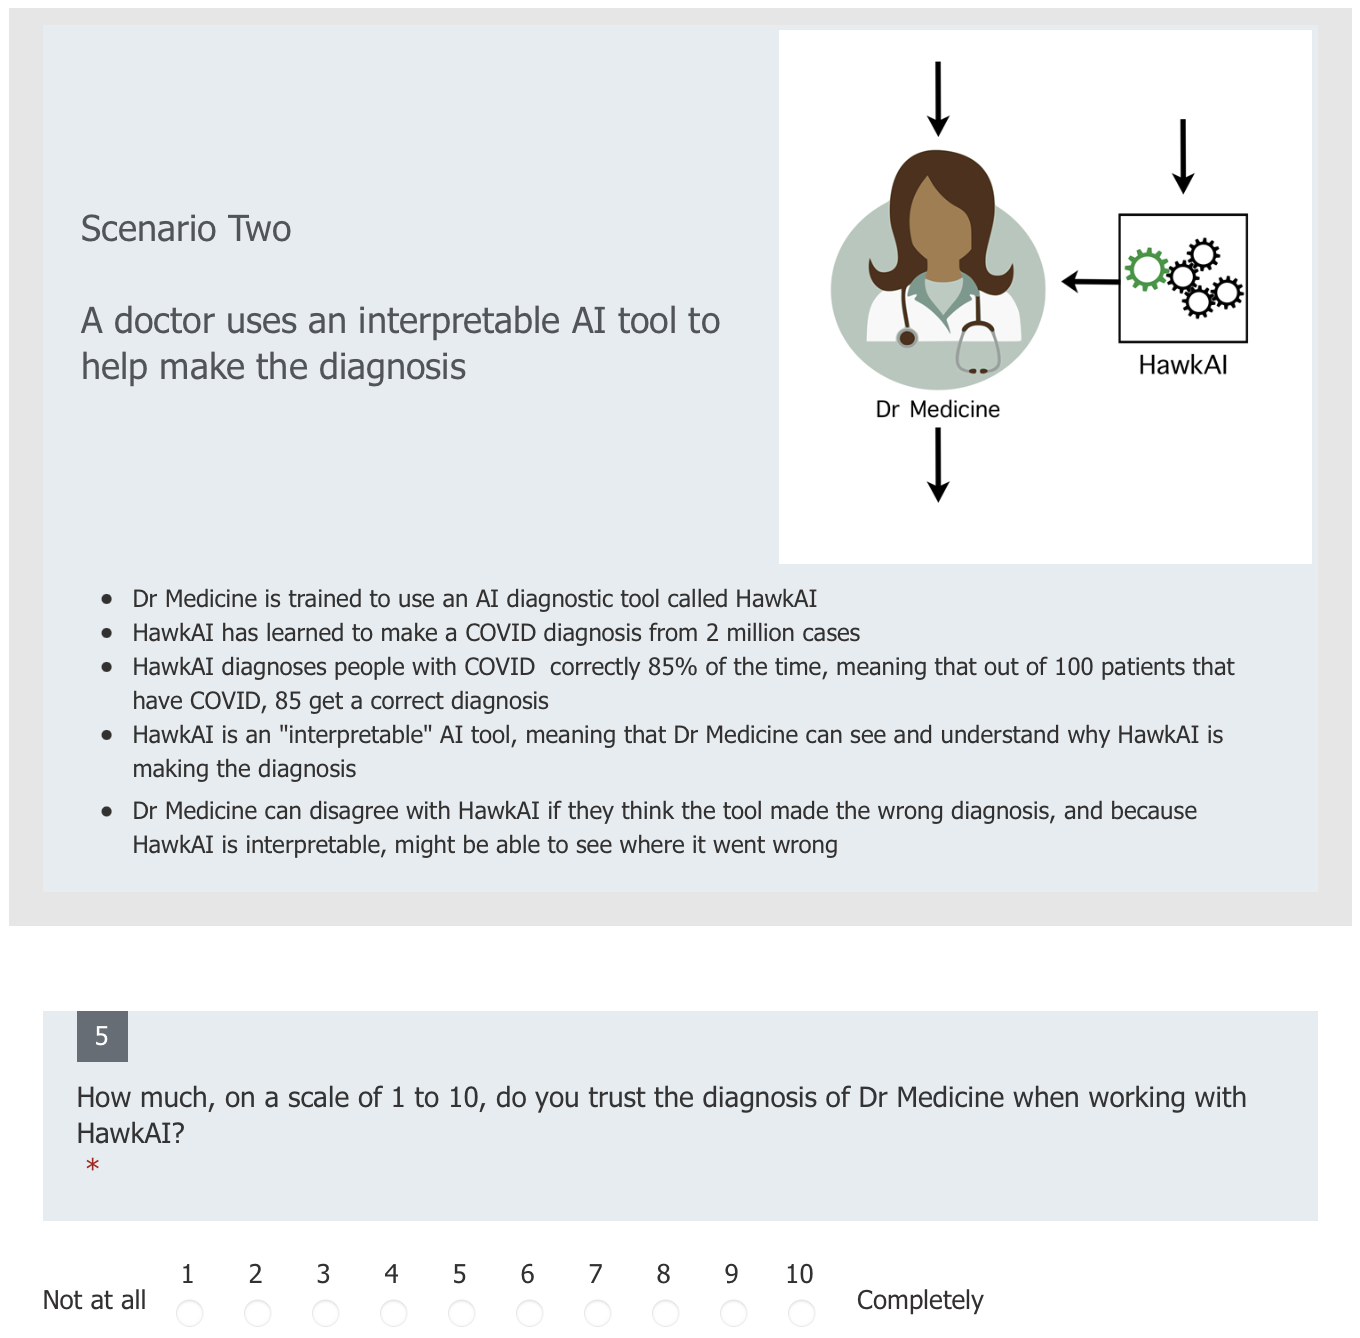
\includegraphics[width=0.75\textwidth]{graphics/Example_survey.png}}
    \caption{Study 1 - Survey Example Question}
  \label{fig:example_survey_question}
\end{figure}

\subsubsection{Ethical Considerations} 
\label{study1_ethics}

When surveying a population, several key ethical considerations must be addressed. Table \ref{table:study1_ethical_considerations} lists these considerations and the actions taken by the research team to address each consideration.

\begin{table}[h]
\begin{center}
\begin{tabular}{ | p{3cm} | p{11cm} |}
\hline
 Ethical Consideration & Action \\
 \hline
 \hline
 Appropriate inclusion and exclusion criteria & The research team excluded minors and anyone who may be mentally or emotionally vulnerable when recruiting from personal networks. Due to the anonymity of participant submissions, recruitment from online platforms (Twitter, LinkedIn, Facebook) could not be monitored and we therefore performed recruitment with the assumption that these organisations have acceptable use policies and appropriate restrictions on age within their terms of service.\\
 \hline
Informed Consent & An information sheet (which can be accessed here: \href{https://sway.office.com/czpQAaqDZiPdpGrB?ref=Link}{https://sway.office.com/czpQAaqDZiPdpGrB?ref=Link} was provided to each participant, detailing the research and any potential risks. To begin the survey, participants were presented with the following message:

\begin{quote}
    By clicking "Next" you confirm that you've read the full information about this study and consent to participate.
\end{quote} \\
 \hline
 The safety and well-being of any participants & In accordance with the University of Bristol ethics approval process, Table \ref{table:study1_risks} identifies physical, psychological, legal and social risks associated with our research and any actions taken to mitigate these risks. \\
\hline
The protection of any participants data & All data was anonymised, with no identifiers included in the questionnaire. A separate email database was recorded for compensation of those who completed the questionnaire. \\
\hline
Compensation & The survey took an average of approximately seven minutes to complete. To compensate participants for their time, each participant was given the opportunity to enter their email address into a separate database (ensuring anonymity) to be entered into a prize draw for one of two £25 amazon vouchers. \\
 \hline
\end{tabular}
\caption{Study 1: Ethical Considerations}
\label{table:study1_ethical_considerations}
\end{center}
\end{table}


\begin{table}[h]
\begin{center}
\begin{tabular}{ | p{6cm} | c | p{6cm} |}
\hline
 Risk & Likelihood & Mitigation \\
 \hline
 \hline
 Physical: None & N/A & N/A \\
 \hline
 Psychological: People might start to worry about their job safety or the quality of a diagnosis based on computer-aided decision-making tools should they require actual diagnosis in future. People might feel bad about themselves not knowing much about computer-aided decision-making tools. & Low & The survey is clearly hypothetical; it does not mention a concrete diagnosis and we clearly ask people to imagine being a patient. The survey does not explore or mention computer-aided decision-making tools replacing people's jobs. The survey will be designed to use simple ways to talk about computer-aided decision-making tools to ensure a wide range of people can understand the questions. \\
 \hline
 Legal: : None & N/A & N/A \\
 \hline
Social: Risk of being identified through combining multiple quasi-identifiers. & Low & Survey data is submitted anonymously. Careful consideration of collected potential quasi-identifiers to ensure minimal chance of identification through combining multiple quasi-identifiers. Exclusion of collecting any non-essential data such as sex, place of work etc.\\
\hline
\end{tabular}
\caption{Study 1: Identifiable Risks to Participants}
\label{table:study1_risks}
\end{center}
\end{table}





% add details on how we requited participants, how many responded and where from.


\subsection{Study 2 - Focus Group}

This section details the focus group which was carried out subsequent to collection of survey data in Study 1. Section \ref{study1_intentions} outlines the intended outcomes of his study.

Section \ref{study1_recruitment_datacollection} details the recruitment and data gathering process and Section \ref{study2_ethical_considerations} outlines any ethical considerations which were to be addressed prior to hosting the focus group session.

\subsubsection{Intention of Study}
\label{study2_intentions}
The intention of this study was to gather qualitative data on participants sentiments towards AI, and to test any hypotheses drawn from the data gathered in Study 1. Study 1 identified semi-distinct preferences for specific demographics within survey participants concerning levels of trust for varied levels of transparency; the focus group format was used to investigate these demographic-specific preferences to ascertain whether any unified reasoning existed within these demographics.

\subsubsection{Study Design}
\label{study2_design}
 
A focus group study followed from the Study 1, to gain insight into the reasoning and motivation behind survey responses, and to uncover topics of interest and concern as well as differences in opinion surrounding AI decision support tools.\\ 

The focus group format was chosen for this phase of research as a suitable means of analysing the maximum number of viewpoints within the scope of the research project time frame. In contrast to individual interviews, where we would be limited to sequentially updating our hypotheses between interviews, the focus group format enables conflicting opinions or theories to be scrutinised in real-time, allowing us to assess the cohesion between different demographics. Additionally, a focus group is an efficient means of maximising researcher contact time for the largest number of participants. We divided the focus group into four distinct segments:
\begin{enumerate}
    \item Introductions and Overview
    \item Sentiment towards AI
    \item Performance vs Transparency
    \item Application Context
\end{enumerate}

The focus group utilised the interactive audience participation tool, Mentimeter, to present the slides in an effort to improve participant engagement and expand interactive functionality \cite{Mayhew2020}. Segment 1 provided us an opportunity to ensure all participants were familiar with the purpose of the focus group and had consented to participate. Segment 2 was designed to allow for a largely unstructured conversation regarding sentiment towards AI. We utilised some interactive elements such as a live word cloud (Figure \ref{fig:word_cloud}) to enable people to present their initial thoughts when considering the term "AI". We used a "conversation wheel" (Figure \ref{fig:conversation_wheel}) to create new topics for discussion and to steer the direction of the conversation when discussion veered off topic or became stagnant.\\

Segment 3 asked participants to rank the four levels of transparency defined in Table \ref{table:transparency_levels} by order of preference, after which the results were presented and used as a prompt for discussion. Finally, Segment 4 asked participants to consider different contexts for application of AI tools and to communicate where any contexts would or would not necessitate higher levels of transparency.

\begin{figure}[h]
       \centering
     \begin{subfigure}[c]{0.48\textwidth}
         \centering
        %  \fbox{%
         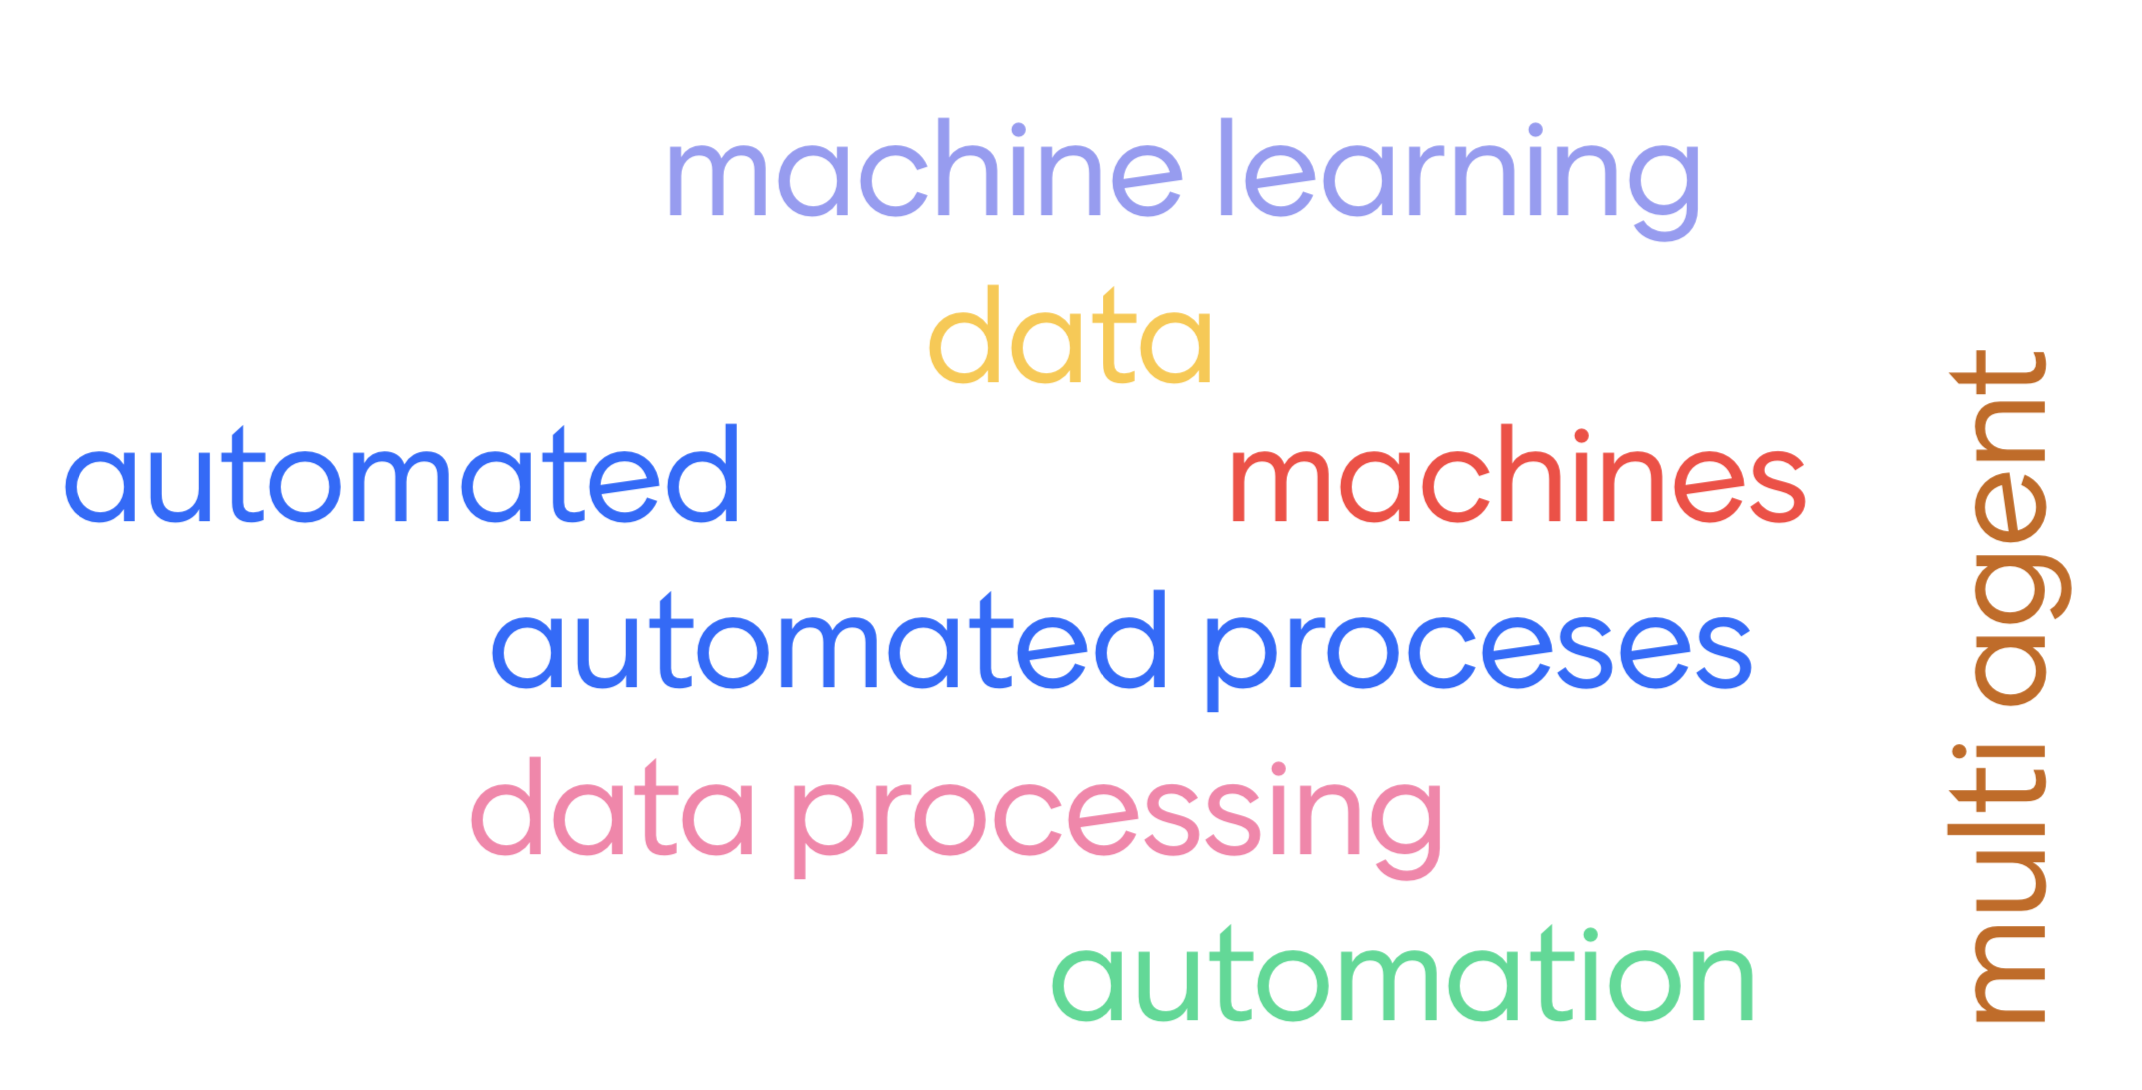
\includegraphics[width=\textwidth]{graphics/word_cloud.png}
        %  }
         \caption{Word Cloud}
         \label{fig:word_cloud}
     \end{subfigure}
     \hfill
     \begin{subfigure}[c]{0.48\textwidth}
         \centering
        %  \fbox{
         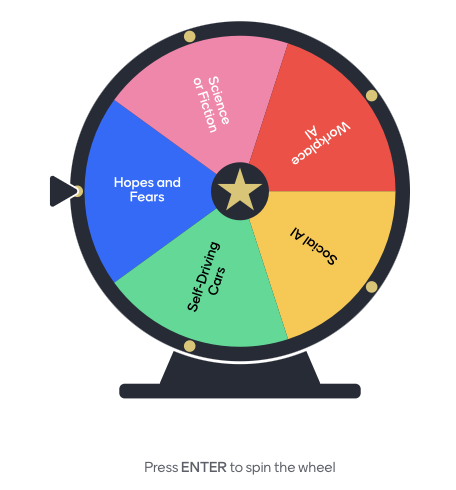
\includegraphics[width=\textwidth]{graphics/conversation_wheel.png}
        %  }
         \caption{Conversation Wheel}
         \label{fig:conversation_wheel}
     \end{subfigure}
     \caption{Study 2 - Mentimeter Interactive Functionality}
     \hfill
\end{figure}

\subsubsection{Recruitment and Data Collection}
\label{study2_recruitment_datacollection}
Recruitment for the focus group was driven by the hypothesis that experience with AI tools, high-stakes decisions or medical contexts may shift a participants' viewpoint on the relationship between trust and transparency. To test this theory, we recruited across the entire spectrum. Having identified eight unique profiles, we leveraged our personal networks to match each profile to suitable candidates. Figure \ref{fig:personality_profiles} details each profile and the associated participant pseudonym.

The focus group was conducted via Zoom. The session was recorded, transcribed and anonymised before being analysed.

\begin{figure}[h]
    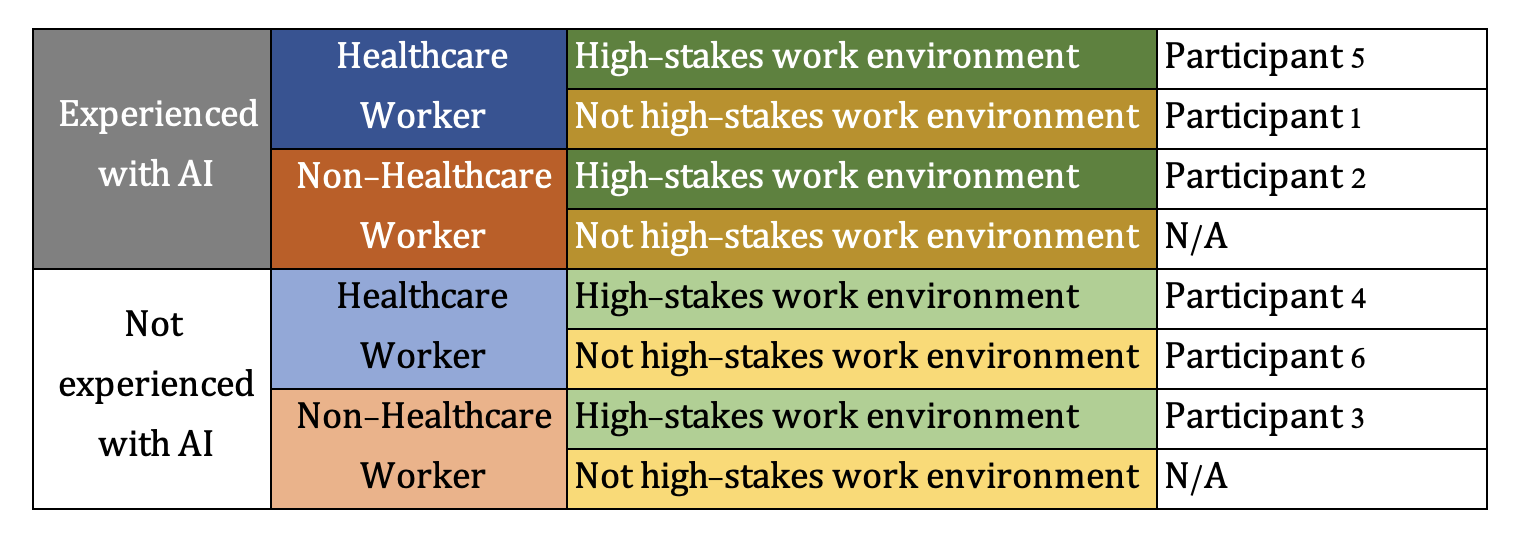
\includegraphics[width=\linewidth]{graphics/personality_profiles.png}
    \caption{Study 2 - Participant Profiles}
  \label{fig:personality_profiles}
\end{figure}

\subsubsection{Ethical Considerations}
\label{study2_ethical_considerations}
 Table \ref{table:study2_ethical_considerations} lists any ethical considerations for the focus group and the actions taken by the research team to address each consideration.

\begin{table}[h]
\begin{center}
\begin{tabular}{ | p{3cm} | p{11cm} |}
\hline
 Ethical Consideration & Action \\
 \hline
 \hline
 Appropriate inclusion and exclusion criteria & The research team excluded minors and anyone who may be mentally or emotionally vulnerable when recruiting from personal networks. \\
 \hline
Informed Consent & An information and consent form (which can be accessed here: \href{https://forms.office.com/r/hup446NJZj}{https://forms.office.com/r/hup446NJZj}) was provided to each participant, detailing the research and any potential risks. Participants were asked to confirm consent before taking part in the focus group. \\
 \hline
 The safety and well-being of any participants & In accordance with the University of Bristol ethics approval process, Table \ref{table:study2_risks} identifies physical, psychological, legal and social risks associated with our research and any actions taken to mitigate these risks. \\
\hline
The protection of any participants data & The recording of the transcript was stored securely on private university-hosted servers, transcribed and the transcription anonymised. Such steps ensure no identifiable information is contained in the final project data repository. A separate email database was recorded for compensation of those who completed the focus group. \\
\hline
Compensation & The focus group required participation for one hour. To compensate participants for their time, each participant was given the a £10 amazon voucher. \\
 \hline
\end{tabular}
\caption{Study 2: Ethical Considerations}
\label{table:study2_ethical_considerations}
\end{center}
\end{table}

\begin{table}[h]
\begin{center}
\begin{tabular}{ | p{6cm} | c | p{6cm} |}
\hline
 Risk & Likelihood & Mitigation \\
 \hline
 \hline
 Physical: None & N/A & N/A \\
 \hline
 Psychological: People might start to worry about their job safety or the quality of a diagnosis based on computer-aided decision-making tools should they require actual diagnosis in future. People might feel bad about themselves not knowing much about computer-aided decision-making tools. & Low & The hypothetical nature of the discussions in the focus group were clearly emphasised; it does not mention a concrete diagnosis and we clearly ask people to imagine being a patient. Any discussions about job safety are of important to our findings from the focus group and so it is deemed acceptable as a topic of discussion, with facilitators aware that they may need to push the conversation along if anyone is showing signs of distress. \\
 \hline
 Legal: : None & N/A & N/A \\
 \hline
Social: Risk of participant data/focus group recording becoming public. & Low & Focus group data is recorded and stored securely, anonymised, and the original data deleted.\\
\hline
\end{tabular}
\caption{Study 2: Identifiable Risks to Participants}
\label{table:study2_risks}
\end{center}
\end{table}


\subsection{Data Analysis - Study 1}

\subsubsection{Dis-aggregation and grouping}

The demographic questions at the start of the survey allow us to investigate how different groups attribute trust in the scenario-based questions. We split into three bins for each of the AI expertise and high-stakes questions. 

These bins are:

\begin{itemize}
    \item Low: $(f_{AI}, f_{stakes}) \leq 3$
    \item Medium: $3 < (f_{AI}, f_{stakes}) \leq 7$
    \item High: $7 < (f_{AI}, f_{stakes})$
\end{itemize}
% $1 \leq (f_{AI}, f_{stakes}) \leq 3$, $3 < (f_{AI}, f_{stakes}) \leq 7$, and $7 < (f_{AI}, f_{stakes}) \leq 10$.
We can also use the profiling questions from the survey to dis-aggregate the survey participants into distinct cohorts that are particularly relevant in discussions of AI transparency: 

\begin{itemize}
    \item Medical professional: Answered "yes" to relevant question
    \item AI Expert: Not a medical professional, and AI experience level reported as $\geq 7$
    \item Public (model patient): Neither a medical professional nor an AI expert
\end{itemize}

These are intended to represent the three agents in each cooperative scenario - the doctor being the medical professional, the patient being the public, and the AI expert standing in for the AI.

\subsubsection{Additional Features}

We use the results of the first scenario, the trust in the doctor with no AI component $T_D$, as a baseline to assess the impact of AI-cooperation on diagnosis trust levels. We denote the trust level reported in these cooperative scenarios based on the nature of their model. Scenario two, with the interpretable or "glass box'' model is $T_{GB}$, and scenario three with the "black box'' model $T_{BB}$.

We normalise the survey scale of [1,10] to [0,1] for $T_D, T_{BB}, T_{GB}$, via $T_i \rightarrow (T_i - 1) * (10/9)$, then produce two new features based on the percentage factor change in trust:

\begin{equation} \label{eqn:change_vs_doctor}
    f_i = 100 \cdot (T_i / T_D)
\end{equation}

These features allow analysis of whether participants view the cooperative use of AI as beneficial ($f_i > 0$), neutral ($f_i = 0$), or inhibitory ($f_i < 0$) to the diagnosis. 

\subsubsection{Unsupervised Clustering}

Having disaggregated into profiling features, then analysed the trust levels of these cohorts, we can instead do the opposite. By starting with trust levels and finding distinct groups of how they are distributed, we can construct cohorts based on trust levels, then use profiling features to find the characteristics of these groups.

Insights can be gained into the results of the survey by applying unsupervised methods. These do not rely on any labels or targets, as would be the case in supervised or semi-supervised methods, so avoid many of the biases that such methods would carry. In particular we apply Uniform Manifold Approximation and Projection (UMAP) \cite{McInnes2018} as dimensionality reduction, then Hierachical Density-Based Spatial Clustering And Noise (HDBSCAN) \cite{McInnes2017} as unsupervised clustering on the resulting UMAP embedding. Both UMAP and HDBSCAN use similar methods, and make similar assumptions, so work well in tandem as an unsupervised exploration method.

UMAP makes the assumption that data is distributed on a uniform manifold, but that the data-space is warped. Using this assumption local distance metrics are learnt, then used to construct a distance graph of the data. A lower-dimensional embedding is then formed, which aims to conserve the form of the high-dimensional space, using a stochastic graph layout. HDBSCAN, similarly, constructs a minimum spanning tree based on distances in the data-space, then applies various sub-algorithms to find clusters. Full explanation of these algorithms is beyond the scope of this work, so the reader should consult the relevant papers for more information. 

\subsection{Data Analysis - Study 2}
\label{study2_data_analysis}

The pseudonymised focus group transcript was subject to thematic analysis; participant contributions were systematically coded by two of the authors, by labeling with meaning, context and theme. The coded statements were then collated and used to synthesise descriptive and analytical themes. The suggested themes were reviewed independently by all authors prior to collectively reviewing their implications to agree upon the central themes emerging from the data.    



\newpage
\section{Findings - Survey}
%Describe our findings from user research
%Evaluation of our findings
%\subsection{Survey}

% \subsection{Dis-aggregation and grouping}

% The demographic questions at the start of the survey allow us to investigate how different groups attribute trust in the scenario-based questions. We split into three bins for each of the AI expertise and high-stakes questions. 

% These bins are:

% \begin{itemize}
%     \item Low: $(f_{AI}, f_{stakes}) \leq 3$
%     \item Medium: $3 < (f_{AI}, f_{stakes}) \leq 7$
%     \item High: $7 < (f_{AI}, f_{stakes})$
% \end{itemize}
% % $1 \leq (f_{AI}, f_{stakes}) \leq 3$, $3 < (f_{AI}, f_{stakes}) \leq 7$, and $7 < (f_{AI}, f_{stakes}) \leq 10$.
% We can also use the profiling questions from the survey to dis-aggregate the survey participants into distinct cohorts that are particularly relevant in discussions of AI transparency: 

% \begin{itemize}
%     \item Medical professional: Answered "yes" to relevant question
%     \item AI Expert: Not a medical professional, and AI experience level reported as $\geq 7$
%     \item Public (model patient): Neither a medical professional nor an AI expert
% \end{itemize}

% These are intended to represent the three agents in each cooperative scenario - the doctor being the medical professional, the patient being the public, and the AI expert standing in for the AI.

\subsection{Mean Results}

To understand the survey results at their simplest we can look at their group averages. Figure \ref{fig:mean_survey_results} shows the mean trust levels for each scenario for our 3 demographic characteristics: AI expertise, medical and high stakes decision makers. We see that on average the Doctor and glass box has the highest trust level, the doctor on their own has second, doctor and black box third and black box on its own fourth. 

When grouped by AI expertise, higher levels of expertise lead to more trust in the cooperative scenarios. No expertise leads to more trust with the doctor on their own and less trust with either black box scenario. Interestingly, the high AI expertise group trust the black box on its own the least. 

Grouping into medical professionals produces no significant trust differences across the four scenarios compared to the rest of the participant population. However, Figure \ref{subfig:high stakes} shows that the greater the high stakes decision making, the more trust is placed in the black box on its own scenario.

\begin{figure}[ht]
  \begin{subfigure}[t]{.45\textwidth}
    \centering
    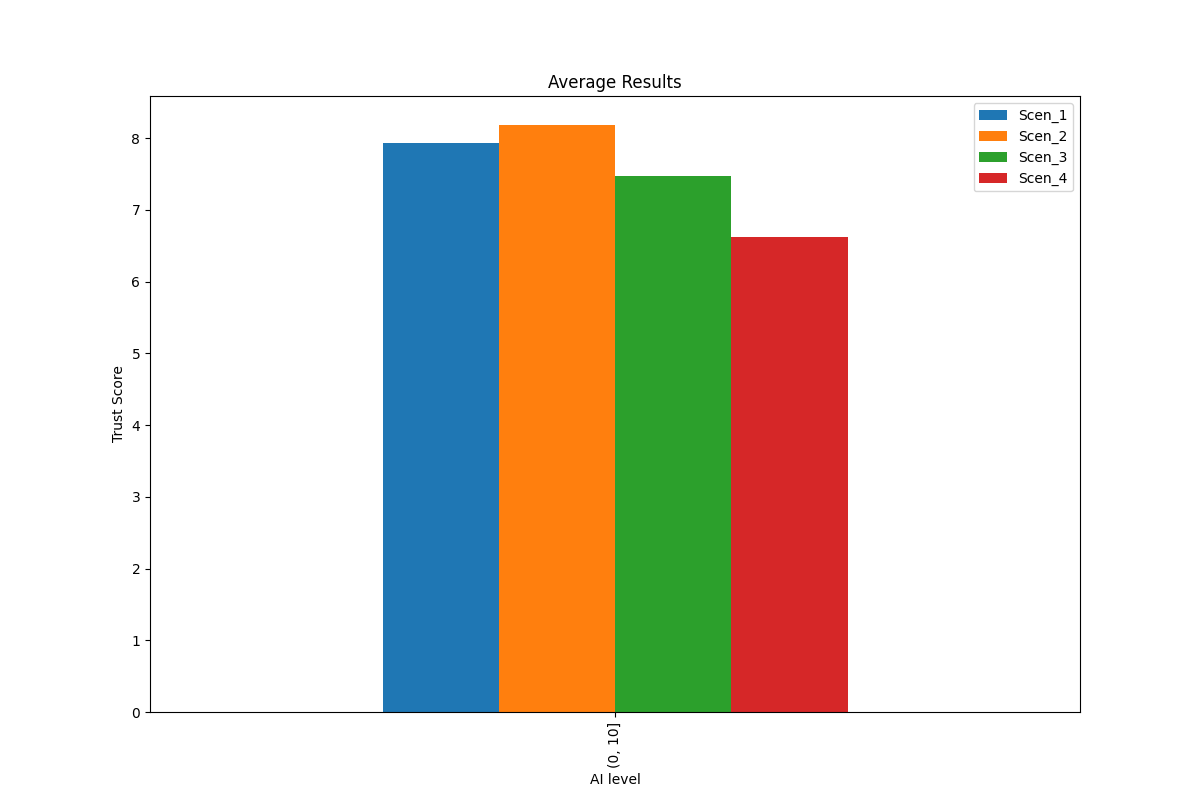
\includegraphics[width=\linewidth]{graphics/survey_averages/survey_average.png}
    \caption{All demographics.}
  \end{subfigure}
  \begin{subfigure}[t]{.45\textwidth}
    \centering
    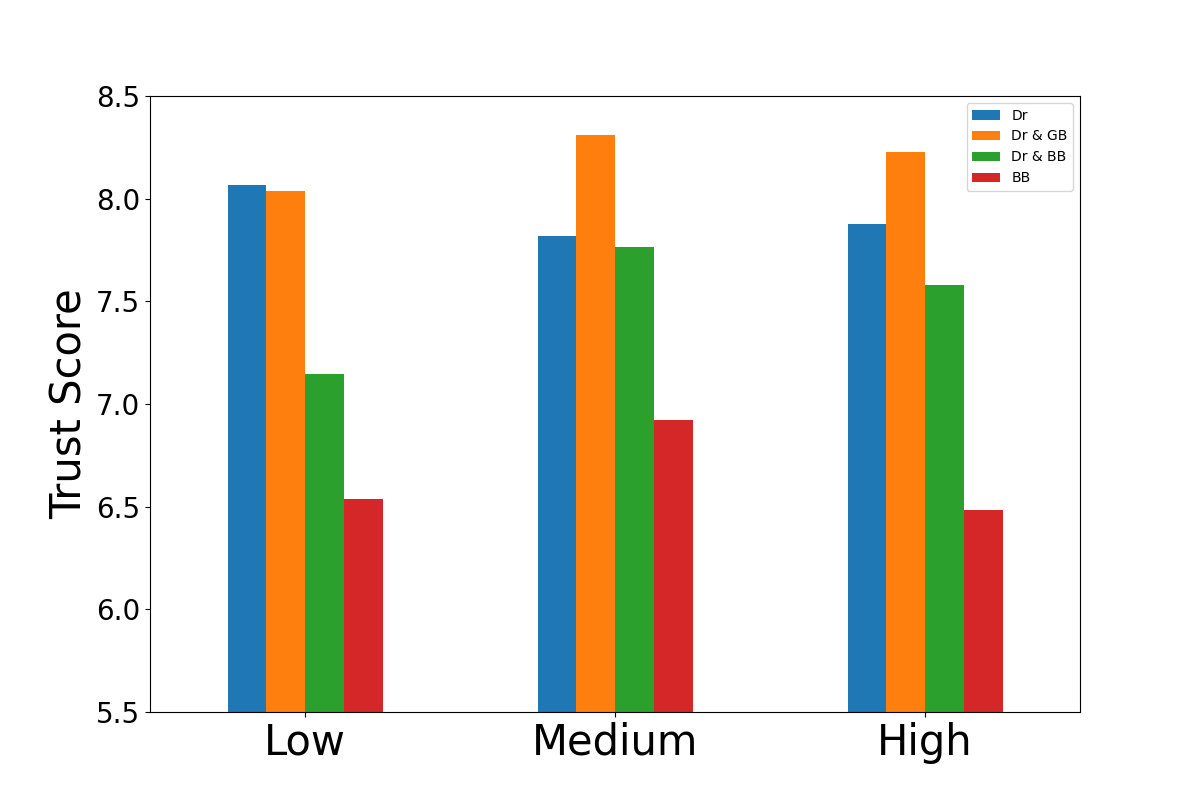
\includegraphics[width=\linewidth]{graphics/survey_averages/survey_AI_grouped.png}
    \caption{Grouped by AI expertise.}
  \end{subfigure}
  \medskip
  \begin{subfigure}[t]{.45\textwidth}
    \centering
    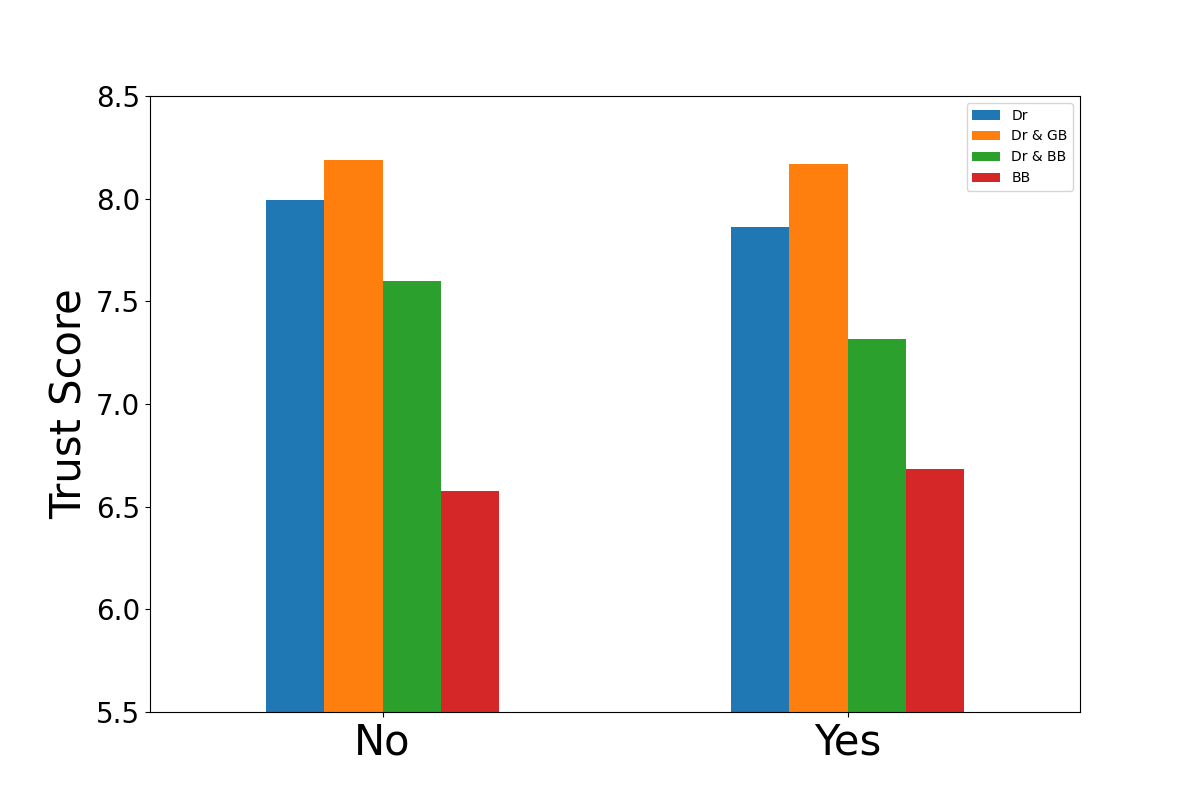
\includegraphics[width=\linewidth]{graphics/survey_averages/survey_medics_grouped.png}
    \caption{Grouped by medical professional.}
  \end{subfigure}
  \begin{subfigure}[t]{.45\textwidth}
    \centering
    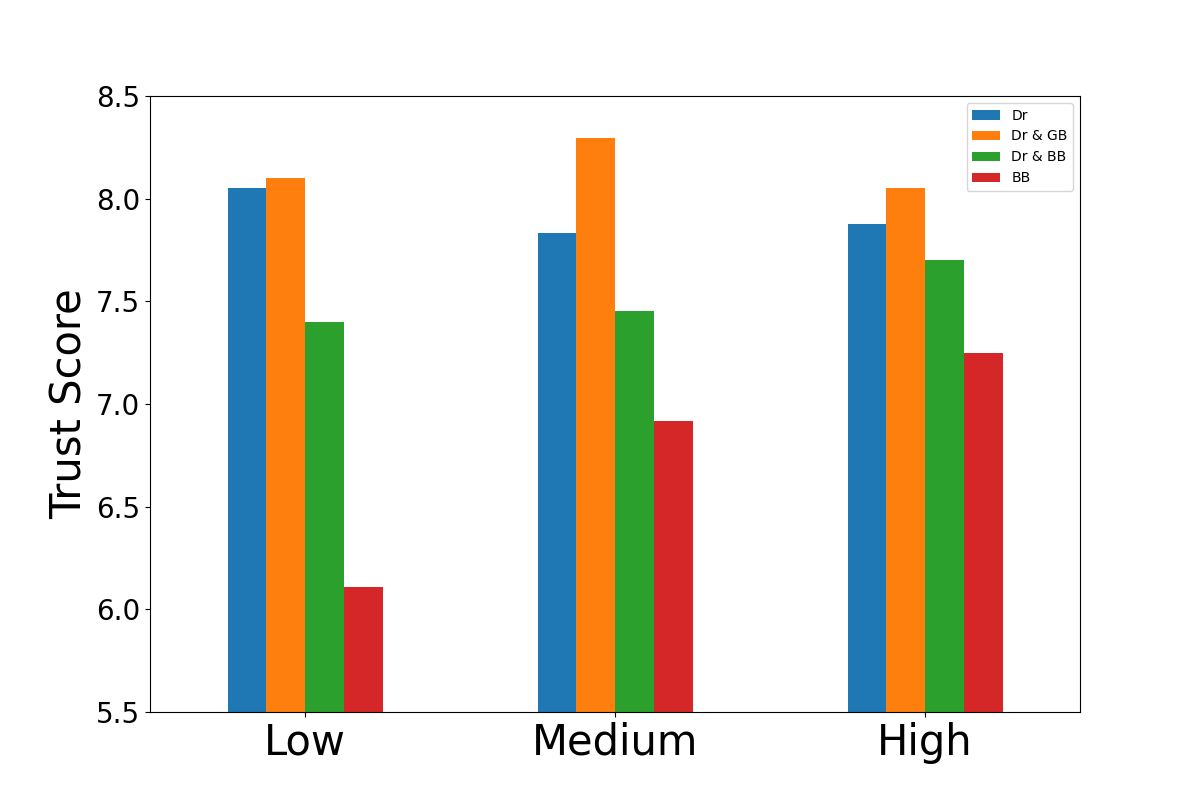
\includegraphics[width=\linewidth]{graphics/survey_averages/survey_stakes_grouped.png}
    \caption{Grouped by high stakes decision making.}
    \label{subfig:high stakes}
  \end{subfigure}
  \caption{Mean results of demographics from the survey results for each 4 scenarios. AI expertise and high stakes decision making numerical values are binned at: Low (0, 4], Medium (4, 7], High (7, 10]. All of the plots use the following colour scheme. Blue: Scenario 1 (doctor on their own), Orange: Scenario 2 (doctor with glass box), Green: Scenario 3 (doctor with black box), Red: Scenario 4 (black box on its own).}
  \label{fig:mean_survey_results}
\end{figure}

\subsection{Scenario Ranking}


Using each participant's trust level in each scenario we are able, for each participant, to rank their scenario preference. We also group using the demographic bins detailed above. The ranking was calculated using pandas' rank function, with ties in ranking resolved using pandas' `average' method\cite{mckinney-proc-scipy-2010}.

In total there were 9 participants who have given each scenario the same number of trust, 49 who have given each scenario a different number of trust, 105 who have given two scenarios the same trust and 115 who have given three scenario the same trust.  To be able to compare the charts across groupings, regardless of how many people are in which group, the proportion of answers is normalised to a percentage of that group with that ranking: $100*(N_{\textrm{Rank}}/N_{\textrm{In Group}})$\%

%number of answers/(total number of answers)*100.

% For AI experience and frequency of high-stakes decision making the rating from 1-10 was binned into three bins: Low, Medium, High using panda's cut function\cite{mckinney-proc-scipy-2010}. The resulting bins are both were low $(0.991, 4.0] <$ medium $(4.0, 7.0] <$ high (7.0, 10.0].

From Fig. \ref{fig:overall-ranking} we can see that the black box (BB) was most frequently ranked the lowest whereas the glass box together with the doctor (DR+GB) was most frequently ranked highest.

While the actual percentage of ranking has to be taken with a pinch of salt given that only 49 participants have given each scenario a different trust level and with it a different rank. The average method used to resolve such ties impacts the number of participants e.g ranking the BB lowest but it does not impact that no matter what the tie resolution strategy is the BB gets the lowest rank.

The black box by itself is, regardless of tied-rank resolution strategy, the lowest ranked scenario.

It is interesting to look at each of the ranks 1-4 and the order in which the different scenarios are appearing in that rank:

For the lowest rank - a ranking of 1 - the BB was by far the lowest ranking scenario followed by the Dr on their own, then the black box with the doctor. The glass box with the doctor was  least frequently ranked the lowest, see figure\ref{fig:overall-ranking}.

For the highest rank - ranking of 4 - the glass box with the dr was ranked most often the highest, the Dr on their own second most often, the black box with the Dr third most often and the black box on it's own was ranked least often the highest, see figure\ref{fig:overall-ranking}.

\begin{figure}[H]
    \centering{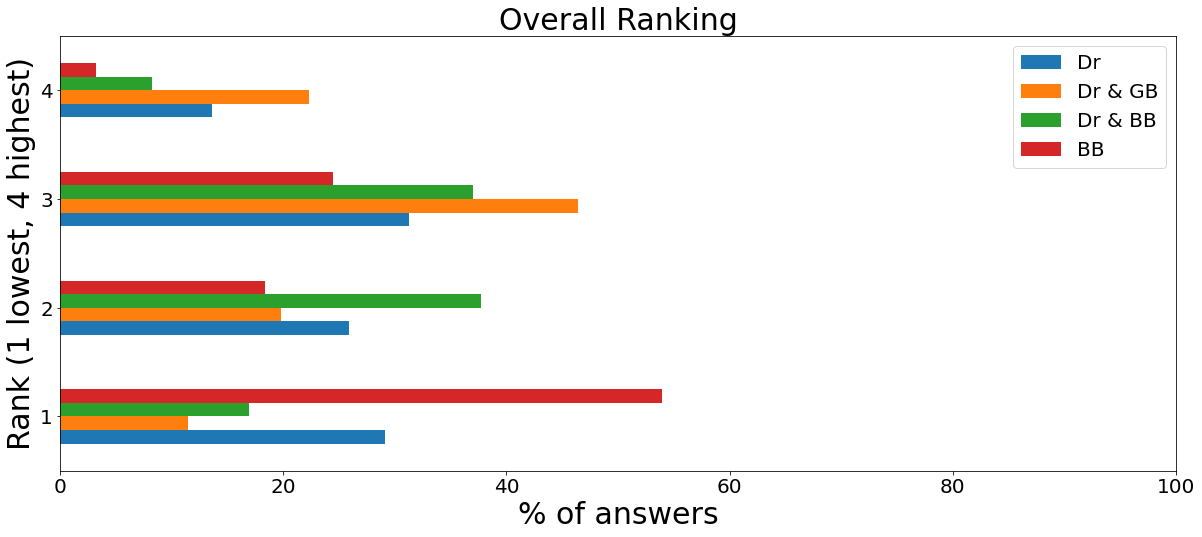
\includegraphics[width=0.8\textwidth]{graphics/ranking/rankingOverallNormalisedAvarageTies.png}}
    \caption{Overall ranking for each of the four scenarios. Rank 1 is the lowest, rank 4 the highest ranking.}
    \label{fig:overall-ranking}
\end{figure}

Looking at how the ranking changes based on if the participant works in healthcare or not we can see that the order for the highest rank (4) and lowest rank (1) stay the same as for the overall chart. However we can also see that people who work in healthcare more frequently rate the Dr on their own as the second most frequent rank(1), see figure\ref{fig:ranking-healthcare}.

\begin{figure}[H]
    \centering{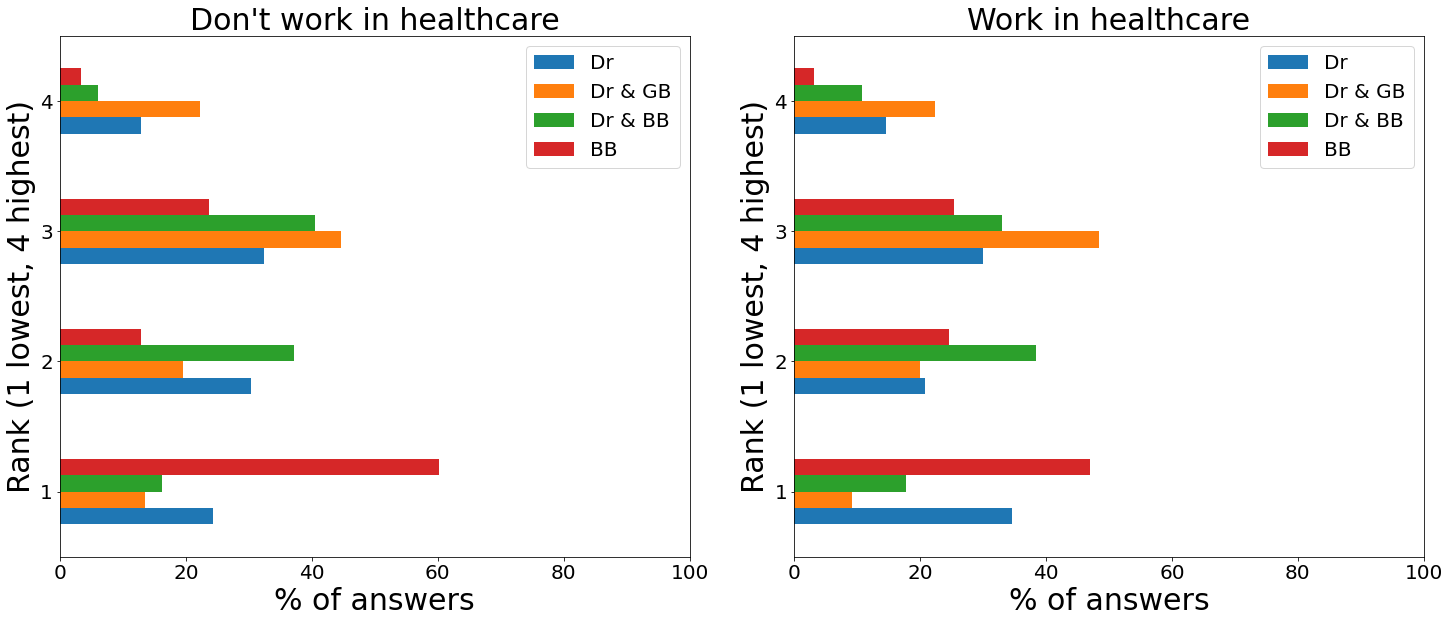
\includegraphics[width=0.8\textwidth]{graphics/ranking/ranking-healthcare-vs-notNormalised-average-ties.png}}
    \caption{Ranking based on participants working in healthcare or not for each of the four scenarios. Rank 1 is the lowest, rank 4 the highest ranking.}
    \label{fig:ranking-healthcare}
\end{figure}

If we look at how the ranking changes with regards to how much AI experience the participants have we again see no change compared to the overall ranking for the highest and lowest rank. We can however see that black box together with the doctor is more frequently ranked in rank 3 for participants with medium and high AI experience and that the black box on it's own is more frequently getting a rank 3 then the Dr on it's own does\ref{fig:ranking-ai}.

\begin{figure}[H]
    \centering{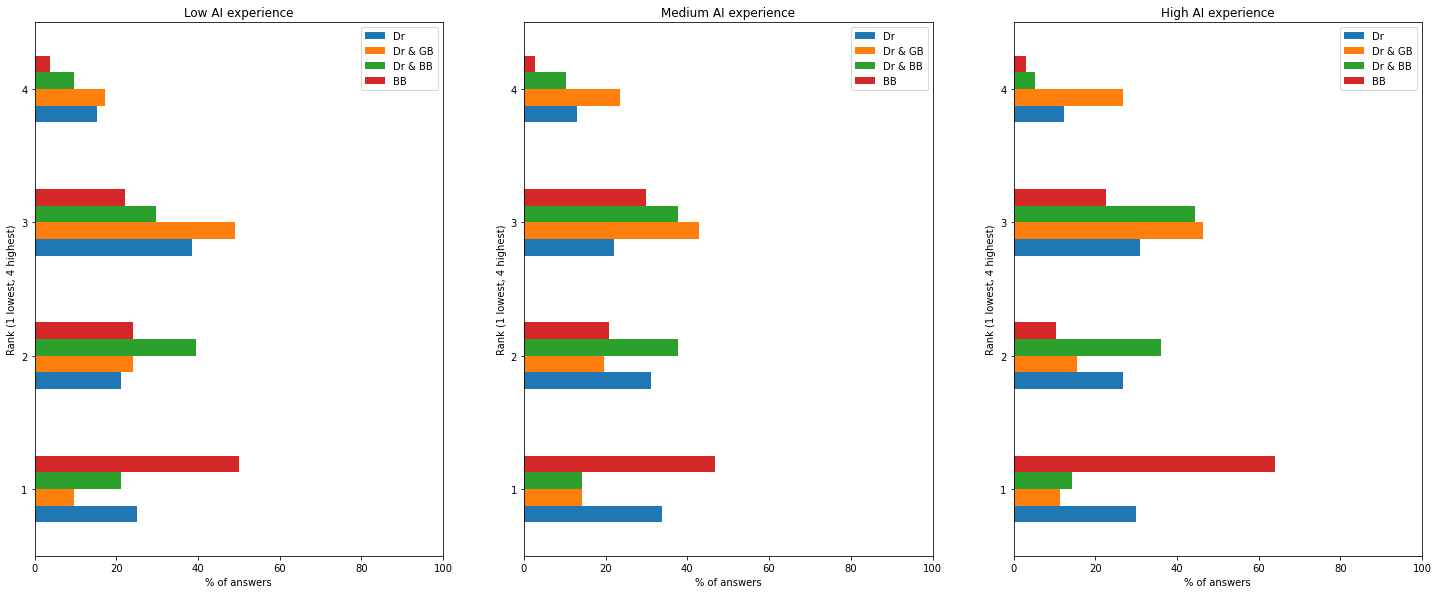
\includegraphics[width=0.8\textwidth]{graphics/ranking/ranking-ai-experience-normalised-average-ties.png}}
    \caption{Ranking based on participant's AI experience of low, medium or high experience for each of the four scenarios. Rank 1 is the lowest, rank 4 the highest ranking.}
    \label{fig:ranking-ai}
\end{figure}

Finally if we look at how the frequency how often a participants makes high-stakes decision changes which scenario gets ranked lowest or highest we can see a change in the high high-stakes decision maker compared to the overall ranking. High high-stakes decision maker rank the Dr on their own as the lowest trust scenario and the black box on its own as the second lowest lowest trust scenario\ref{fig:ranking-highstakes-decision}..

\begin{figure}[H]
    \centering{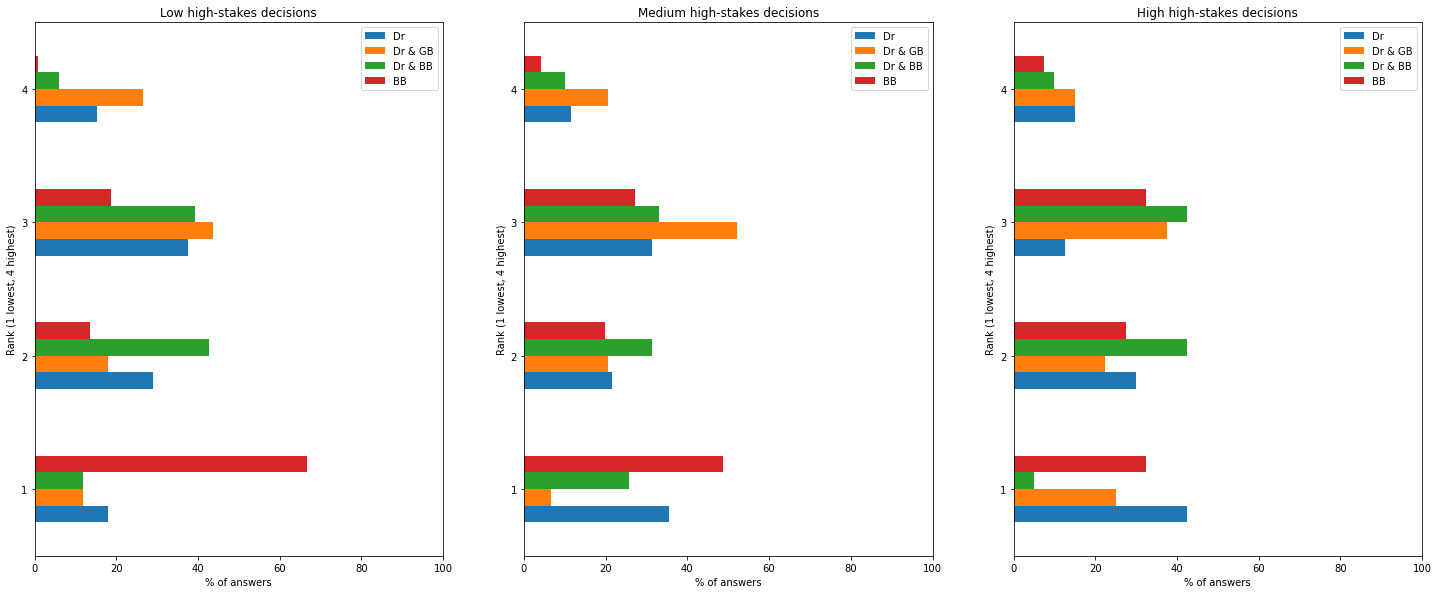
\includegraphics[width=0.8\textwidth]{graphics/ranking/ranking-high-stakes-decisions-normalised-average-ties.png}}
    \caption{Ranking based on participant's frequency of high-stakes decision making of low, medium or high frequency for each of the four scenarios. Rank 1 is the lowest, rank 4 the highest ranking.}
    \label{fig:ranking-highstakes-decision}
\end{figure}

% \subsection{Data Analysis Survey}

% /JE

% Highlight the use of covid diagnosis makes people apply the risk to themselves. So we get more thoughtful/emotive responses.

% Split into Study one and Study two.
% How did we pick the 5 people from the focus group





%AD





\subsection{Demographic Motivated Impact of AI}

%=======================D

% \subsubsection{Additional Features}



%=======================D

% We plot the results in Figure \ref{fig:improvement}, along with an interpretation schema, with participants dis-aggregated into three cohorts given the following criteria:



% The survey was closed after XXX days, with XXX participants. We use the two key profile features - AI experience level and whether the participant is a medical professional - to dis-aggregate into three demographic bins:


We apply Equation \ref{eqn:change_vs_doctor} and analyse the changes in participant trust in the two doctor/AI cooperative scenarios using Figure \ref{fig:improvement}.

\begin{figure}[h!]
    \centering
    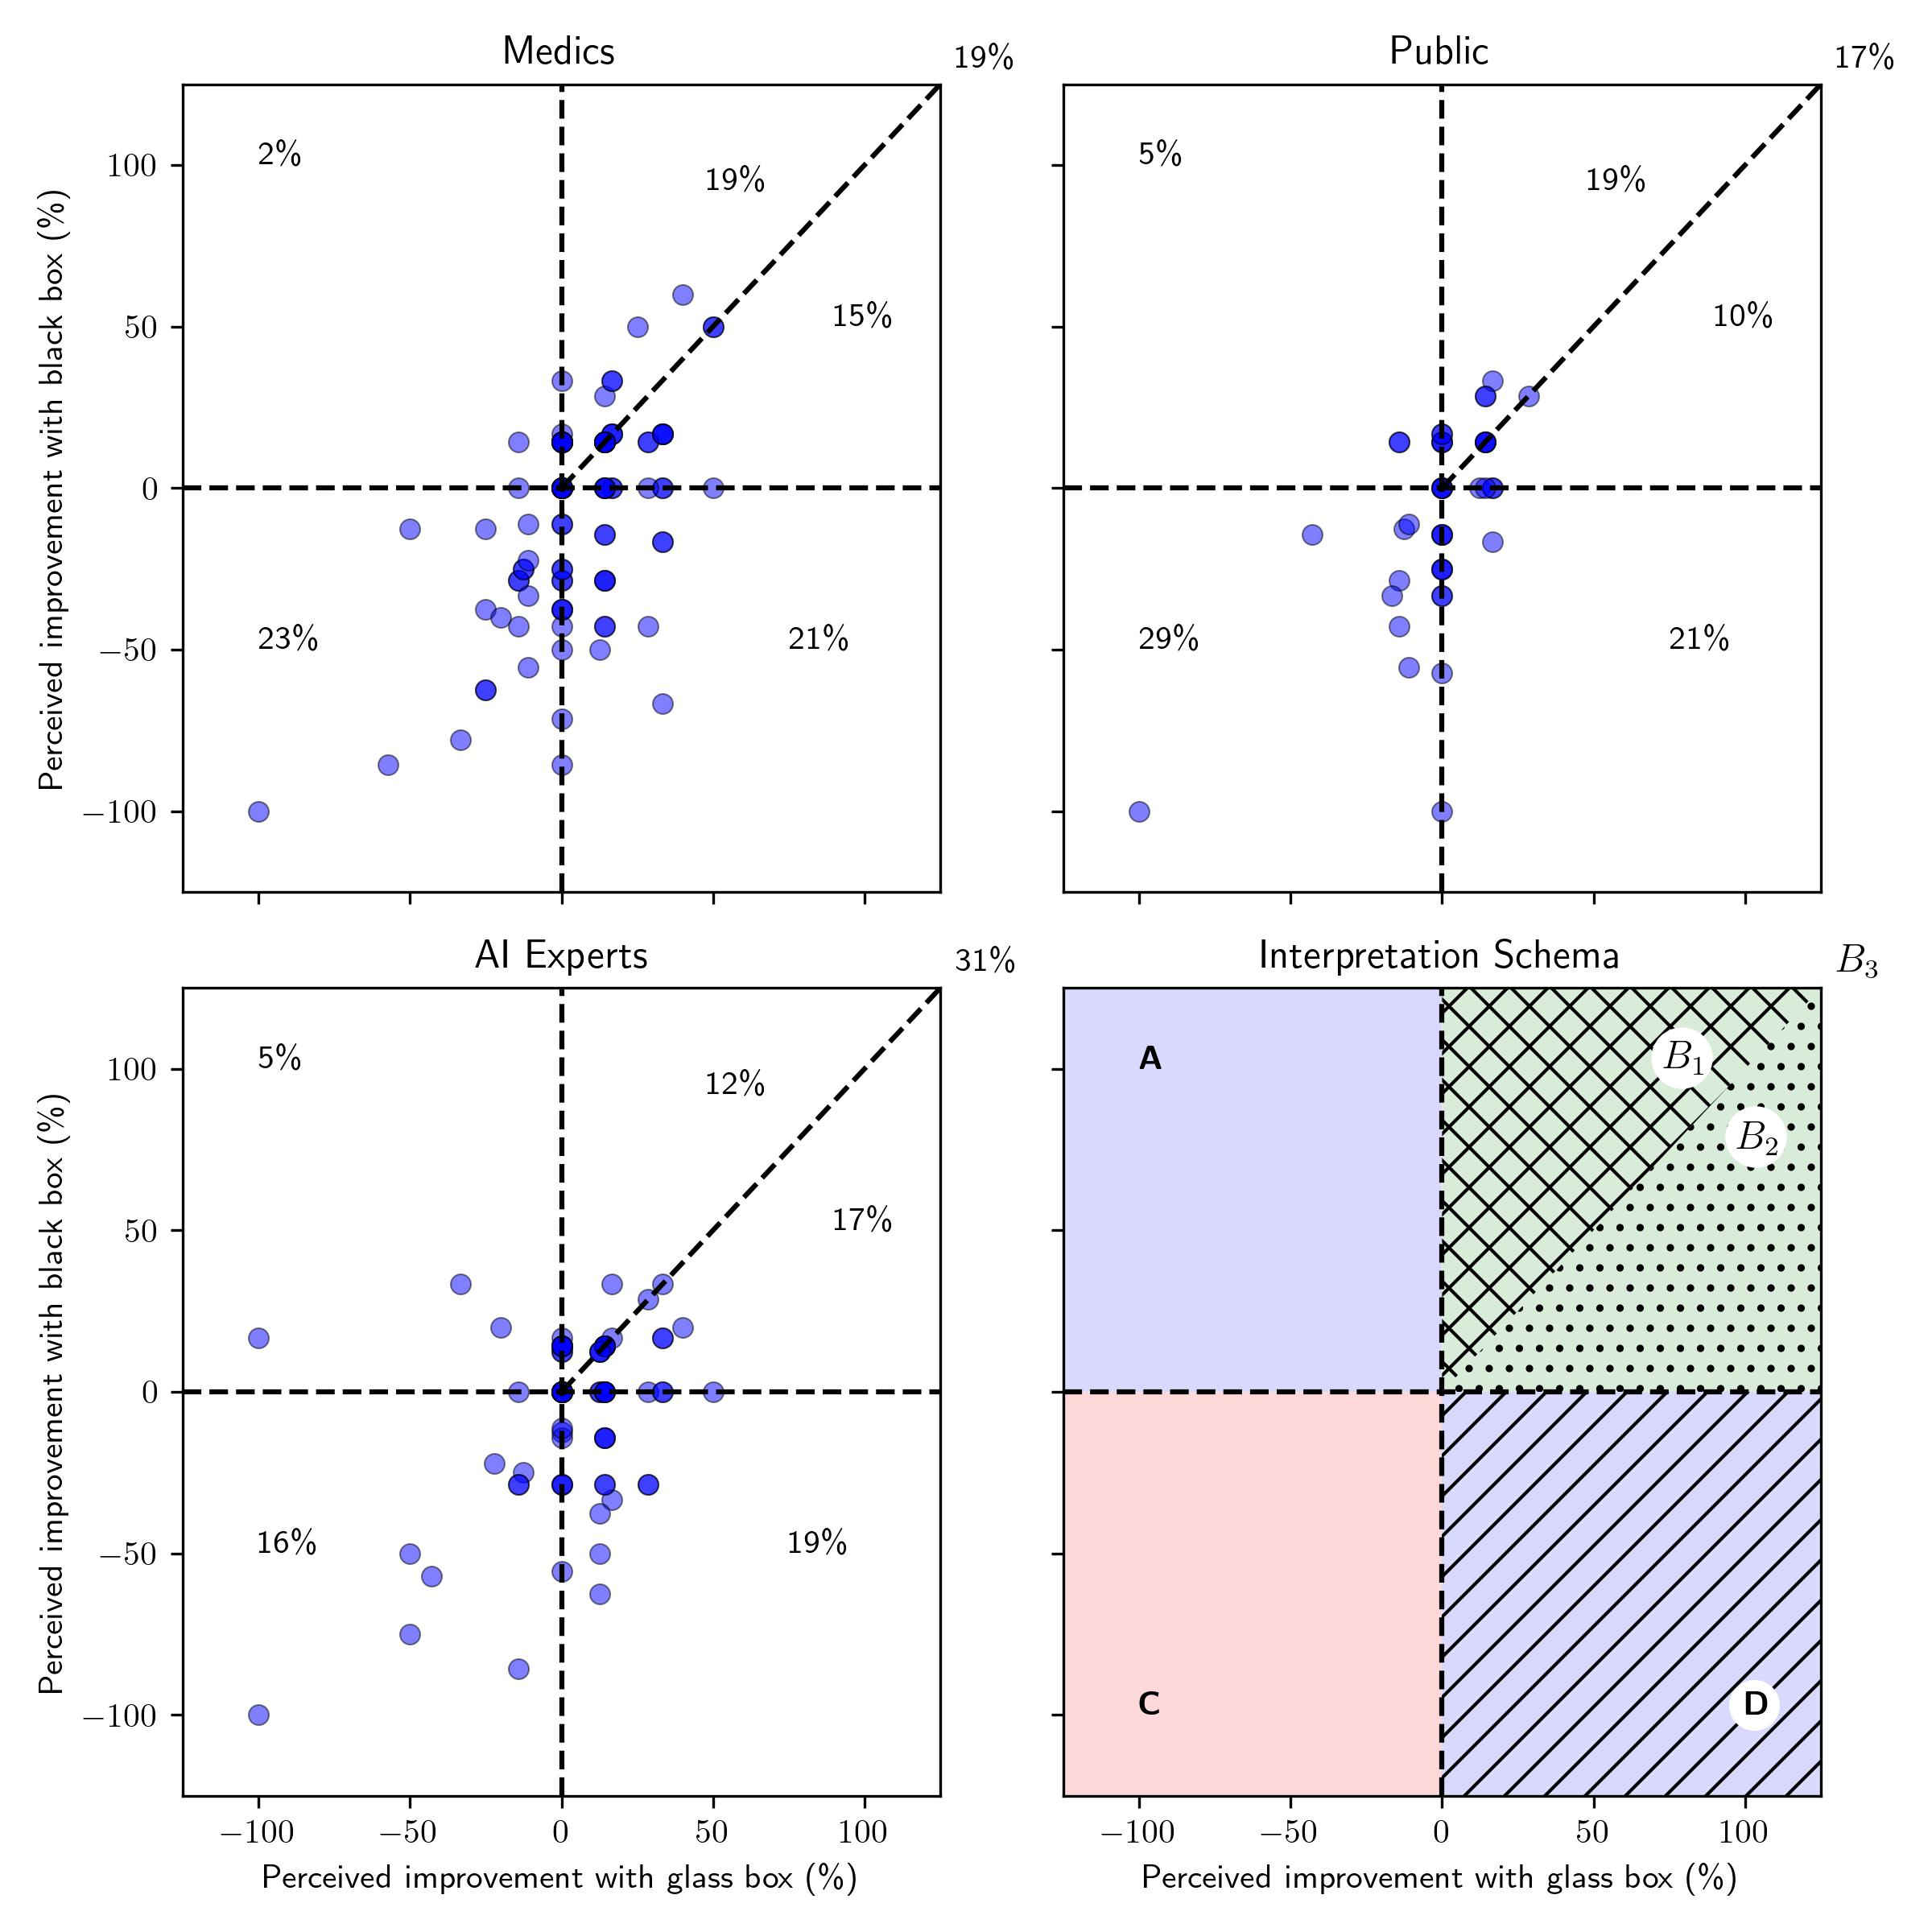
\includegraphics[width=0.85\textwidth]{graphics/Doctor_improvements_cooperation_scatter.jpg}
    \caption{\centering Perceived improvements in trust in scenarios 3 and 4. Percentages are calculated using $\leq 0$ and $>0$ basis.\hspace{\textwidth} Interpretation schema: \textbf{A}: Black box improves diagnosis, glass box makes diagnosis worse \hspace{\textwidth} \textbf{B}: Both glass box and black box improve diagnosis. \textbf{$B_1$} black box is preferred, \textbf{$B_2$} glass box is preferred, $B_3$ neither is preferred. \textbf{C}: Neither glass box nor black box improve diagnosis \textbf{D}: Glass box improves diagnosis, black box makes diagnosis worse}
    \label{fig:improvement}
\end{figure}

Through Figure \ref{fig:improvement} we derive how different cohorts view the use of AI in cooperative scenarios. In all cohorts, a significant proportion of participants view the use of AI as beneficial with both models - 46\% of the public, 53\% of medical professionals, and 60\% of AI experts. This can be assumed to match the progression of technical expertise between cohorts.

Only a minority of each cohort view neither AI-cooperative scenario as beneficial. In all cohorts the glass box model is preferred over the black box model, but only by a small margin, with ratios $f_{BB}:f_{GB}$ of 1:1.17, 1:1.125 and 1:1.40 for the public, medical professionals and AI experts respectively. Table \ref{tab:demographic_trust_change} shows the percentages from Figure \ref{fig:improvement}.

\begin{table}[h]
\begin{tabular}{c||c|c|c}
     & Public & Medics & AI Experts \\
     \hline \hline
    GB and BB inhibit (C)            & 29\% & 23\% & 16\%\\ \hline
    GB inhibits, BB improves (A)     & 5\%  & 2\%  & 5\% \\
    GB improves, BB inhibits (D)     & 21\% & 21\% & 19\%\\  \hline
    GB and BB improve (B)            & 46\% & 53\% & 60\%\\ \hline
    GB and BB improve (equal)        & 17\% & 19\% & 31\%\\
    GB and BB improve (GB better)    & 10\% & 15\% & 17\%\\
    GB and BB improve (BB better)    & 19\% & 19\% & 12\%\\ 
\end{tabular}
\caption{\label{tab:demographic_trust_change}Perceived changes in trust of a diagnosis from an AI/doctor cooperation, dis-aggregated into previously described demographics. Note: Relevant percentages may not sum to 100\% due to rounding errors.}
\end{table}
%\subsection{Correlation Analysis}

Using Table \ref{tab:demographic_trust_change} we can see a more subtle dynamic in participant trust ratings by inspecting the proportions of each cohort that view both cooperative AI scenarios as improving the diagnosis. The proportion that view both glass box and black box as useful increases with presumed technical level (public, medics then AI experts). However AI experts who view both scenarios as beneficial to the diagnosis are less likely to favour the black box compared to the glass box. Adding to this, as presumed AI technical expertise increases (again public, medics, then AI experts), the proportion explicitly favouring the glass box scenario also increases.

This analysis has shown that across all cohorts at least some version of doctor-AI cooperation is seen as beneficial to a diagnosis, with only a minority of each cohort viewing both presented scenarios as inhibitory to assigned trust. These proportions, 29\%, 23\% and 16\% for the public, medics and AI experts respectively, decrease with presumed level of technical expertise. Similarly, the proportion of participants in each cohort that view both cooperative scenarios as beneficial to a scenario follow presumed technical expertise, with 46\%, 53\% and 60\% for the public, medics and AI experts respectively.

\subsection{Trust Motivated Clustering}



We apply UMAP, then HDBSCAN to the resulting embedding, and present the results in Figures \ref{fig:embedding}, \ref{fig:cluster_means}. UMAP produces four distinct clusters, which are recognised by HDBSCAN. HDBSCAN is designed to find clusters in noisy data, and so can identify points as noise, but none are found here, indicating that clusters are clearly defined.

\begin{figure}
\centering
\begin{subfigure}{0.5\textwidth}
  \centering
  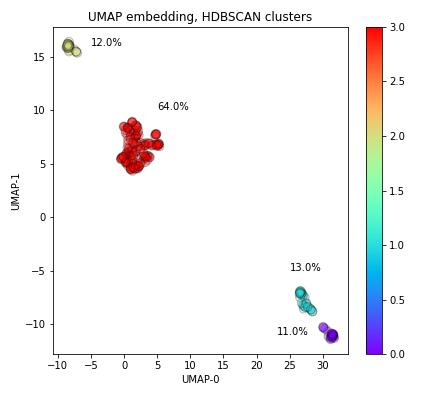
\includegraphics[width=\linewidth]{graphics/UMAP_HDBSCAN.jpg}
  \caption{}
%   \caption{The UMAP embedding produces four (visually) distinct clusters, which are also identified by HDBSCAN.}
  \label{fig:embedding}
\end{subfigure}%
\begin{subfigure}{0.55\textwidth}
  \centering
  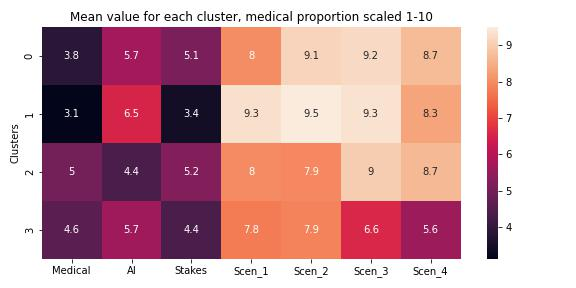
\includegraphics[width=\linewidth]{graphics/clustering_means.jpg}
  \caption{Cluster means across all four scenarios, along with profiling features.}
  \label{fig:cluster_means}
\end{subfigure}
\caption{The results of unsupervised clustering with UMAP and HDBSCAN. In Figure \ref{fig:cluster_means} profile features (AI, Medical, Stakes) are normalised by the whole population. Scenario trust levels are moved to a scale [0-1] for greater clarity in the heatmapping.}
\label{fig:test}
\end{figure}

The clusters identified by this process are distinct in how the participants within them rated trust in the different scenarios. Clusters 1 and 3 follow the same trend, with the highest trust in the glass-box cooperative scenario, and lowest in the solo black-box. However, cluster 3 has significantly lower trusts across all scenarios. Cluster 3 is significantly larger than the other clusters, representing 64\% of the participant pool.

Clusters 0 and 2 have the lowest level of trust placed in the doctor, with the solo black-box scenario scoring higher, in contrast to the opposite relationship in clusters 1 and 3. In both cluster 0 and 2 the highest trust is in the black-box cooperative scenario. Cluster 2 is the only cluster in which the glass-box cooperative scores lower than the solo doctor.

This analysis of only prescribed trusts leads to an intuitive split: In evaluating the compromise between transparency and efficacy, those in clusters 0 and 2 prescribe more weight to efficacy, and those in clusters 1 and 3 weight transparency over efficacy. Those in cluster 0 are perhaps closer to even balancing of transparency and efficacy than those in cluster 2, as shown by their higher trust levels in the glass-box scenario.

Cluster 1 probably represents a population of AI researchers - high average AI knowledge, but low stakes decision making and a small medical proportion. These participants rate any doctor-lead scenario highly, and only show a significant decrease in trust when a doctor is not presented as making the final decision, as in scenario 4.

Cluster 2, which leans the most towards following efficacy statistics, has the highest proportion of both medics and high-stakes decision makers. This might indicate that the cluster is composed principally of medical professionals, who are likely to rate themselves as more frequently making high-stakes decisions. This would also explain why this cluster has the lowest average self-reported AI knowledge compared to the whole survey population.

Clusters 0 and 3 are less easily identified, but might represent different subsets of the general population. Cluster 0 has a higher self-reported stake level, but a lower than average medic proportion, so might represent high-stakes decision makers from outside the medical field. Cluster 3 is very close to the average in all three of our profiling features, and is the largest, so could be said to represent the public, or the equivalent for our participant pool.


\newpage
\section{Findings - Focus Group}

This section details the findings from thematic analysis of the transcript from the focus-group session, comprising several recurring themes from the discussion, and statements relevant to the results of the survey study. 

% The pseudonymised transcript was divided into individual statements, which were independently systematically coded by two of the authors, by labeling with meaning and context. The coded statements were then collated and used to synthesise descriptive and analytical themes. The suggested themes were reviewed by independently by all authors, before meeting to discuss their implications, and to agree upon the central themes emerging from the data.    

Whilst the focus-group was designed to encourage discussion about the subject of trustworthy AI in any context, discussion tended to remain focused on a clinical context unless otherwise prompted.

Statements associated with each of the six participants are labeled as P1-P6. 


\subsection{Performance of AI is Important, Detailed Information is Needed}
When evaluating the trustworthiness of the example scenarios given in the survey study, some participants may have made their decision based entirely on the stated performance. In this context, this was a single value indicating the average percentage of patients that would be correctly diagnosed by either the doctor, glass-box or black-box systems in isolation. Some participants of the focus outlined a compatible belief, that the system which has the best performance is the one they would trust the most. 

P6 “I think it said in the survey that the black box had a higher percentage [accuracy] than the human, so I'm pretty sure that I put it higher than just the human as well”

P1: “I think all of this is based around how accurate the black box is.” 

The above statements appear to be made on the assumption that the stated performance is consistent across demographics and future use cases.

P6 suggests later in the discussion that a single overall performance metric may not be sufficient information to secure trust in an AI system due to difference in performance over different demographics “One of the biggest things is how good the performance is depending on the group of people that it is assessing. I'm guessing that we are assuming that it is the same across the board i.e. diagnosing women or men or children and adults. I guess that is good because you could be like “performance is worse for children, and this is a child so maybe we have to take that into consideration”“. 

P5 identifies the importance of understanding the data on which a model has been trained -
 “The AI is only as good as the data it's got and if it's not got a lot of data for a certain minority or gender or children then it won't perform well there”. Transparency in terms of explainable AI may not be needed to address this issue if information regarding how the black-box system was developed and trained is provided, as well as performance statistics broken down by demographic.


\subsection{Low Transparency may Cause Susceptibility to Bias} 
Several participants demonstrate awareness of the implications of opaque AI - a user cannot know how an algorithm or AI system can make a decision.

P6  "if whoever is using the algorithm doesn’t understand how it reaches those decisions then I guess it can reach the wrong decisions and no one will know and there is no way of catching that." 

P1 [on AI in the context of phone app recommendations]  "ultimately, it decides what those apps are going to be and it may not be influenced by my decisions. It may be choosing those based on whatever it likes, I have no idea".

P6 discusses how a lack of transparency can make it difficult to address bias in the context of black-box systems: “I guess it's hard because with the black box you don’t know how it has reached its decision, so you don’t know what sort of biases are going to be in the system”....”in an ideal work you'd know that black box was taking in all the different information that it needed to. Especially I think in terms of minorities which have a history of not having that much data. So, I think that’s one element of having the human there that they could take that sort of information into account when maybe the black box doesn’t.“

P2 raises concerns around AI systems introducing or perpetuating social bias - "I think there was one [example] about insurance, where if your name was [X] then your insurance was multiple time higher than if your name was [Y] That is the fear side of it, the more we allow those sort of decisions to be made by people called [Y] then that’s great because all the [Y]'s get cheap insurance but that’s where my fear lies.



\subsection{Transparency Less Important for Low-Stakes Contexts}

P1 [on AI in targeted advertising and social media] - ''Honestly, it doesn’t really bother me. If I'm getting targeted ads that are for me, you know I don’t want to get adverts for things that I don’t need in my life. So, it doesn’t bother me that much.''

[Quote in response from P5 suggesting there may be more issues with low-stakes scenarios as well regarding data protection]

P1 describes a scenario in which, for low stakes decisions, a lack of explainability and transparency can be beneficial due to it’s convenience. "My phone knows what app I want to use before I even do. I open my phone and it says “do you want to use [App]?” and I'm like yeah I do, I don’t know how you know that but I do. So in that sense I think that it’s a really positive thing, and I think that it makes organisation a lot easier. But there are definitely scary parts to it". 

There is a trade off here, where the user may be willing to relinquish control and autonomy in return for convenience and utility for low-stakes applications. 

When asked if there were circumstances where an autonomous blackbox system may be appropriate in healthcare, P4 responded described a low-stakes clinical scenario “I think something more like minor ailments is more appropriate and you do see that quite a bit with online pharmacies, they have sites available for minor things that you wouldn’t have to go to a GP for like UTI. You just go through a bunch of questions and tick your symptoms, how long you’ve had it and all the safety questions. But to be fair that does get reviewed by a doctor at the end of the line before everything gets signed off. But if something had a high accuracy rate then that wouldn’t, to me, be much of a problem, if the patients been given all the relevant information.”. 

\subsection{Transparency Required for Higher Stakes Contexts to Address Accountability}
Later in the discussion, when discussing the use of AI for identifying criminal suspects, P2 expresses that it may be reasonable to require transparency as we would for a human decision maker in the same context:  “Say for example you as a human being say: “I've looked at the evidence and I think we should get X in for some questioning”. If the computer said the same thing, you'd want to know the evidence that gave it that conclusion. We'd want an analogous process. Rather than it be a black box, you want to know why. It feels like that’s the bit that you'd want for machines to be trustworthy.”

P1 echoes this sentiment later in the discussion with respect to the clinical scenario from the survey by comparing doctors and blackboxes: “...aren’t doctors black boxes anyway? I don’t know what their thought process is”... “they can give you their evidence for it but how often do we ask: “how did you get to that diagnosis?” Most patients just accept it at face value”. 

P4, a healthcare professional involved in some diagnostic and other clinical decision making, explained their perspective on why transparency is necessary. “I think that I'm really adverse to relying solely on [a decision making system for which] you can't tell how that decision is made. More like an accountability type thing if something goes wrong. How can you explain to that patient or their family if you don’t really know how it came to that decision”. 

When asked who’s at fault when an AI draws the wrong conclusion, P3 responded “Can you blame a robot? I don’t know?”.


\subsection{Transparency Less Important if there Is Justifiable Need, However there Are Concerns to Be Addressed}

P2 “if you could scale up the diagnosis and allow it to be quicker and earlier, then that could be a really valuable thing for me to trust in a black box, at least for a first port of call. Say for example I could install an app on my phone where I could take a picture everyday and you could tell me if I've got covid, that for me could be low stakes or could be high stakes, but that gets rid of the onset of it all and do all those horrible tests. If something like that was a computer and could give me a 90% accuracy or even say “you look a bit jaundiced, you should probably go to a doctor” that feels like a really valuable use of a black box technology. 

P3 “The problem with hospitals or GPs is that there is not enough staff and too many patients so something like that would speed up the process where people can’t see a GP. “... “I guess sending pictures of yourself to this unknown thing in the internet, you want to know where those pictures are going any what they are being used for. “

\subsection{Importance of Transparency and Human Interaction for Patient/User Experience}
P3 “I think in certain stuff like healthcare people want a personal touch, they want someone there. For me even if I'm doing a PhD in AI, I'd like someone there to talk to me about things. Because you always tend to have questions and follow ups and if you just have an AI make a decision then it might not be that transparent. “

P3 “it comes back to what someone was saying earlier with the emotional side of work and everyday life... Does there need to be a human touch?”

P2 “I was just thinking about what if you are on the wrong side of the decisions and how that makes you feel. What if I go to doctor and they misdiagnose me, I think would be more forgiving than if a computer misdiagnoses me. Because I think a human is more fallible.”

P5 “I probably would be more forgiving to a doctor than a black box. And I think if a doctor can give a reason for why they’ve picked that then it might make sense to me. I think the same thing with the glass box where I can see why it thought that rather than just giving an answer.”

\subsection{The importance of transparency and human accountability may be greater for higher stakes scenarios}

P2: “Well if it’s a terminal diagnosis or something like that that feels like you couldn’t leave that to a computer, right?”... “I wonder how people would feel? If there was a black box that said “you have cancer and you have 6 months to live”. 

P4 identifies that a human is required to convey and discuss certain results to a patient, and that an autonomous AI system may not be appropriate - “You’d have to be really sensitive to what that patient actually would benefit from knowing. Some people don’t have the capacity to know the full amount, some people might have other things going one, whereas a human doctor can pick up on the nuances of that and gauge the reactions, especially when it is breaking bad news like that.” P4 confirms that they “think it’s really important actually” to have at least a human interface for delivering information, even if the information is produced by an AI system. 

In practice, a human healthcare professional will always be responsible for the care of a particular patient or service user. This responsibility includes acting in the interests of patients safety and wellbeing, and upholding the interests of vulnerable individuals in how care is delivered. 

P2 “if you're going to tell that by adding in a computer that it’s going to get more accurate, even if it’s a terminal diagnosis I'm very comfortable with that, but I'm not sure I'd want just the AI. It comes back to what P4 was saying a bit, as a human being I'm probably going to have quite an irrational response in the first instance to something that life changing and I might say things like “are you sure, how do you know that, can I get a second opinion” and with the black box it feels like none of that is possible.”

\subsection{Design of the Cooperation Between AI and Human Is Important}
Survey findings show that in general, participants ranked scenario (3/C) [black-box with human] higher than scenario D/4 [blackbox alone]. 
Participants of the focus-group discussed why they agreed or disagreed with this trend. One participant explained why they did not perceive that the human in scenario (3/C) improved the trustworthiness with respect to scenario 4/D without the human. 

56 (P6) “I definitely put [black-box] above black box with human”... 
“the human has no way of knowing whether what the black box did was right so why would it disagree with it, so it seems pointless having the human element in there”

Participant 5 responded to this point, and explained their reasoning for thinking that scenario C/3 was more trustworthy than scenario D/4. 

58 (P5) “a black box and human should be better just a black box because... [it's similar to] who wants to be a millionaire where you ask the audience... you get a bunch of statistics, and you can confirm your belief or not”. 
The participant makes the point that the doctor has their own assessment of the situation in addition to the assessment provided by the black-box.

The doctor could use the black-box output as a way of confirming their belief (a kind of second opinion), or to indicate where they may need to review their assessment. Further the participant suggests that the doctor may over time develop an intuition for the kinds of mistakes the black-box will make:
“if they have had past results and background then they’ll know roughly whether it’s accurate or not”.

P2:“it could be that the doctor makes the diagnosis and uses the AI as confirmation rather than a diagnostic itself. The doctor would first parse the information in of what he thinks is pertinent, but I think that there are risks there because you’ve got the human bias in there as well.”

Participant 6 clarifies the reasoning behind their decision by raising valid questions which highlight the ambiguity surrounding the relationship between the  human and AI system within the decision making process.

60-62 (P6)
“is it that the human and the black box makes a decision and they collate? The way I saw it was that the black box makes the decision and the human without any additional information makes a decision separately decided to accept it or not. “
“I guess in an ideal work you'd know that black box was taking in all the different information that it needed to. Especially I think in terms of minorities which have a history of not having that much data. So, I think that’s one element of having the human there that they could take that sort of information into account when maybe the black box doesn’t. “
The human and AI could fit into the wider decision making process in different places and in different ways, which could result in or address different biases.

P2 also highlights that in the survey scenarios, the  - “it could be that the doctor makes the diagnosis and uses the AI as confirmation rather than a diagnostic itself. The doctor would first pass the information in that he thinks is pertinent, but I think that there are risks there because you’ve got the human bias in there as well.”

P1 “If the AI is smarter than the doctor, does it not have the capability to then sway the doctor...?“

If the doctor is aware that on average, the AI system is more likely to be correct than they are, they may be more likely to dismiss their own perspective when it conflicts with the AI system. In some contexts, this could mean that a human working with a black-box AI system could perform worse than either in isolation due to variations in human bias when evaluating the output of the blackbox. 





\newpage
\section{Discussion}
Contribution we've made

%AD - from changes in trust and clustering

\subsubsection{Cooperation (AD), changes:}
\begin{itemize}
    \item AI experts like the AI cooperation scenarios most - 60\% have higher trust than in doctor
    \item If you like the black box, you also like the glass box, and very few in any population only like the black box
    \item AI experts have the smallest proportion liking the glass box and disliking the black box
    \item Disliking both glass box and black box follows AI technical level (descending): Public $\rightarrow$ Medics $\rightarrow$ AI
\end{itemize}

\subsubsection{Clustering (AD):}
\begin{itemize}
    \item Clustering isolates medics and AI researchers
    \item AI researchers follow what we'd expect: they trust AI the most, but weight towards transparency over efficacy, and don't like the black-box working solo
    \item Medics weight heavily towards efficacy, but still rate a doctor having the final decision higher than the black box by itself
    \item General population is split into low/high stakes
    \item High-stakes genpop are less scared of AI, and seem to weight efficacy and transparency equally important, but still want a human final decision
    \item Low-stakes genpop (the actual public?) are scared of AI, especially when its not transparent. They don't like the Terminator doctor, sorry Arnold.
\end{itemize}

%ID - conclusions from Ranking and Literature

\subsubsection{Ranking (ID)}
\begin{itemize}
    \item BB least trusted across demographics
    \item GB+DR most trusted across demographics
    \item the second least trusted scenario was Dr on their own
    \item DR on their own second most trusted scenario
    \item higher stakes decision makers trust the Dr less
    \item medium+high AI expertise trust BB more than the low expertise
    \item from Focus group, dislike of BB has more to do with lack of empathy in the communication not if it is interpretable, transparent or not
    \item from FG high performance is important for BB
\end{itemize}

%MC - from focus group
\subsubsection{focus group (MC):}
\begin{itemize}
    \item preference to doctor or human relaying information
    \item full disclosure of any AI used in a system
    \item performance of AI important
    \item transparancy of AI important for high stakes
    \item low stakes transparancy less important
    \item confusing over who is accountable for AI decsions
    \item second opinion from AI seen as useful over doctor on own
    \item trust issues around data privacy
\end{itemize}

\subsubsection{Overall themes/contrasts (AD):}

\begin{itemize}
    \item There are distinct differences in how people attribute trust, with identified groups having some distinct differences, but not entirely explained by our demographics ("ITS A COMPLEX ISSUE GUYS OKAY")
    \item Preference for AI cooperation increases with technical expertise level
    \item Human-in-the-loop is always preferred - backed up by focus group
    \item Transparency is also important - across all cohorts no one really prefers the higher performance BB coop to more transparent GB coop
    \item Issues of trust from focus group about accountability (who takes the blame? less incentive to have a good process if no human takes the blame?)
\end{itemize}



The use of both demographic-lead and trust-level-lead analysis has demonstrated that the key stakeholders in a high-stakes decision attribute different trust levels to AI-assisted decisions. Unsupervised analysis using UMAP and HDBSCAN identified four distinct families of thought, with the largest of these groups heavily weighted against non-transparent AI. 

This analysis is useful as a way to check whether our demographic features can fully explain the differences in assigned trust - it seems as if they cannot. While each cluster was demographically distinct, it was not to the extent that might be expected. The cluster with the highest average AI expertise was only 10\% higher than the whole population average, indicating that AI expertise does not play an overly influential part in how trust levels differ between these groups. One cluster had a significant proportion of medical professionals - 30\% higher than the whole population mean proportion of medical professionals - and the participants in this cluster actually rated the scenarios with the black-box AI as more trustworthy than other scenarios. This might indicate a result-oriented or efficacy-weighted consideration of the scenarios.

This differed significantly from the largest cluster, who had roughly average demographic features. This cluster - perhaps representing the general perspective and thought on AI decision making tools - had the opposite trend to the cluster with highest medical professionals, rating any black-box scenario as much less trustworthy than transparent AI equivalents. 

Through all analysis of the survey results and from the focus group it is clear that a human should be involved in the diagnosis process.

We find that the perceived benefit of AI-cooperation, essentially using AI as a diagnostic tool, tracks technical level of expertise in our model scenarios. AI experts are the most likely to favour either AI-tool being used in diagnosis, and a majority of medical professionals do the same, but this is not true of the general public. Given that the public as a stakeholder in these scenarios represent the patient, it is worth further discussion of where they do in fact view AI assistance as beneficial.

Responses from the focus group indicate that the level of transparency is indeed significant to trust levels:

\begin{quote}
    \textit{``...if whoever is using the algorithm doesn't understand how it reaches those decisions then I guess it can each the wrong decisions and no one will know and there is no way of catching that"} - P6
\end{quote}

This tracks with survey results from demographic motivated analysis, where significantly higher proportions of all cohorts view the glass-box cooperative scenario beneficial and the black-box as inhibitory than the inverse. However, out of those that view both scenarios as beneficial, only AI experts prefer the glass box.

This would seem to indicate a combined consideration of both the efficacy and transparency of a model, which is a critical concern in AI decision making. The transparency seems to be considered first - hence the universally higher proportions of participants viewing black-box as inhibitory and glass-box as beneficial compared to the inverse - but if a participant views the transparency as a fair trade-off for efficacy, they are more likely to lean towards the high efficacy of our model black-box agent.

Interestingly, despite this, across all demographics the black box by itself is significantly lower than the doctor by themselves. This is backed up with results from the focus group:

\begin{quote}
    \textit{``...I probably would be more forgiving to a doctor than a black box. And I think if a doctor can give a reason for why they’ve picked that} [diagnosis/decision] \textit{then it might make sense to me. I think the same thing with the glass box where I can see why it thought that} [diagnosis/decision] \textit{rather than just giving an answer."} - P5
\end{quote}

\textbf{Isabella can you add a bit here about what the literature says RE: is a glass box actually better than a black box in cooperation with a human? I remember there were a couple of papers saying not necessarily}

Significant proportions of those who view both cooperations as beneficial rated their increased trust equally - see Table \ref{tab:demographic_trust_change}. This, given the lens of a tradeoff between transparency and efficacy, would indicate that those who trust AI-cooperative decisions weight transparency and efficacy equally. 



\newpage
\section{Conclusion}

\begin{itemize}
    \item the more knowledge about AI or the more someone told about AI (in the focus group) the more trust they place in it
    \item glass box helps to increase trust, (focus group said it is closer to human decision making therefore easier to place trust straight away)
    \item performance of AI is important for trust (but might need to be explained why e.g. faster decision or more error from human decision caught in systems under pressure)
    \item glass box systems are preferred even with lower performance (until why performance is important is explained)
    \item we can disprove the papers that say users like doctors and dislike AI *
    \item full disclosure of how AI is used in systems, especially black box ones is crucial for acceptance and trust.
\end{itemize}



%%
%% The acknowledgments section is defined using the "acks" environment
%% (and NOT an unnumbered section). This ensures the proper
%% identification of the section in the article metadata, and the
%% consistent spelling of the heading.
\begin{acks}
Acknowledgments
\end{acks}

%%
%% The next two lines define the bibliography style to be used, and
%% the bibliography file.
\newpage
\bibliographystyle{ACM-Reference-Format}
\bibliography{elf}

%%
%% If your work has an appendix, this is the place to put it.
\appendix

\section{Optional Supplementary Material}

\subsection{Study Ethics}

% DC - Need to go through and format, I've been working in a google doc
% How do I add line space after subsubheading?
\subsubsection{Organisation and Funding}


This work was organised and funded by The University of Bristol School of Computer Science, Electrical and Electronic Engineering, and Engineering Maths.

Investigators are students enrolled on the “Interactive Artificial Intelligence CDT” at the University of Bristol, and are funded by UKRI Studentships.

This work was completed as part of a University course “Interaction Design COMSM0087”, led by Dr Paul Marshall.


\subsubsection{Ethical Approval} 


Ethical approval for study methods described in Section [?] of the report was granted by University of Bristol Faculty of Engineering Research Ethics committee prior to study recruitment.

The study has been reviewed by the unit director, Dr Paul Marshall.

The risks associated with participating in the study were assessed as low likelihood and low severity. 

\subsubsection{Incentive}  


At the recruitment stage, prospective participants were told that there would be a monetary incentive for participation.

For participation in the survey, this was the option to be entered into a raffle to win one of four Amazon gift vouchers worth £25 each.

To facilitate this, participants could opt in to the raffle by providing an email address, which was stored securely on a University server. 

Email addresses were stored separately from survey responses to prevent any reassociated. 

At the time that the survey was closed to new participants, four email addresses were selected at random to receive the vouchers.

Once the selected participants had confirmed they received the vouchers, all email addresses were promptly deleted. 



\subsubsection{Privacy and Data Management}  


Survey:
No personal identifiable information was collected during the survey phase of this work.

Survey data was collected via Microsoft Forms, and stored on a secure server hosted by the University of Bristol.

Participants had the option of providing an email address to opt into a raffle to win a monetary prize. 
This email address was not associated with their survey response, and was used only to send the prize to the relevant participants. 
Email addresses were stored on a secure University of Bristol server and deleted after prizes were allocated.  

Focus Group:
The focus-group was conducted remotely via Zoom online video conferencing. 

The focus-group was recorded for the purpose of transcribing the discussion, and was deleted when the audio had been transcribed. 

All audio transcriptions were pseudonymised prior to analysis.

All data gathered for this work (survey responses, email addresses, focus-group audio, transcript) was stored on a secure University of Bristol server. 

\subsubsection{Recruitment:}  


The total number of survey participants was [XXXX] at the time of closing.
Survey participants were recruited by:
Direct contact
Sharing the survey with personal contacts
Mailbases 
Survey was sent to the directors of the following University programs to be  distributed to the students:
[Which programmes?]
The survey was posted in a medical physics and engineering special interest mailing group: JISCMAIL Medical-Physics-Engineering 
Social media
The survey was distributed through personal Twitter accounts (resulted in about 3 participants) as well as 5300 followers dogs of Twitter account with followers from all over the world and different backgrounds which resulted in over 100 participants.
Participation was open to all members of the public, however recruitment was targeted towards three groups: healthcare professionals, AI/ML specialists, and general public. The studies population is not therefore reflective of a cross-section of the general public or specific demographic groups. 
No demographic information relating to protected characteristics was collected. 
The only objective information requested from participants was whether or not they work as a healthcare professional. 
Six focus-group participants were recruited from personal contacts. 

\subsubsection{Informed Consent Survey}  


Written consent was obtained for the survey study…
A participant information sheet was presented at the start of the survey. Participants were required to confirm that they have read the information sheet before progressing with the survey to ensure informed consent as much as was reasonably practicable. 
I.e. “By clicking "Next" you confirm that you've read the full information about this study and consent to participate.”
The participant information sheet included:
Background about the project and project organisers.
The purpose of the study
Reason participants have been recruited. 
Eligibility criteria
Details of participation:
Emphasis that participation is voluntary
Emphasis that participant can choose to withdraw from the study (relevant to focus group).
Description of how data will be managed and used.
Details of incentive.
Details of confidentiality. 
Emphasis that no personally identifiable information is recorded in the survey. 
Right to withdrawal.
Contact details for asking questions. 
Intended outcomes of the research project.
Eligibility criteria i.e. requirements for participation as specified in the information sheet include:
Participant is over 18 years old
Participant has internet access to participate in online data collection

 
\subsubsection{Informed Consent Focus-Group}  


Participants were sent an information sheet directly, and asked to confirm they had read and understood the provided information prior to the event.

At the start of the focus group session, participants were given the opportunity to say if they had not read or understood the provided information, or if they had any concerns they wanted to raise. 

\subsubsection{Other}  



%Check notes from other group
%Check any other comments/document related to ethics
%So far, I've mostly just looked at the ethical approval document and the details from our information sheet.


% DC - Need to go through and format, I've been working in a google doc
% How do I add line space after subsubheading?


\subsection{Part Two}  




\end{document}
\endinput
%%
%% End of file.
